% This is paper draft
% edited by Haoruo Peng
% Date: 2013.5.27
\documentclass{llncs}
\usepackage{llncsdoc}
\usepackage{amsmath, amssymb}
\usepackage{color}
\usepackage{graphicx}
\usepackage{bbding}

\newcommand{\bw}{\mathbf{w}}
\newcommand{\bwep}{\mathbf{w}^{\varepsilon}}
\newcommand{\bwfly}{\tilde{\mathbf{w}}}
\newcommand{\bwavg}{\mathbf{wavg}}
\newcommand{\bu}{\mathbf{u}}
\newcommand{\buprev}{\mathbf{uprev}}
\newcommand{\bp}{\mathbf{p}}
\newcommand{\bq}{\mathbf{q}}
\newcommand{\bxi}{\mathbf{\xi}}
\newcommand{\dotwxb}{{\mathbf{w}}^{\mathbf{T}}\mathbf{x}_{i}+b}
\newcommand{\sumt}{\sum_{t=1}^{T} }
\newcommand{\lc}{\left(}
\newcommand{\rc}{\right)}
\newcommand{\li}{\lc i\rc}
\newcommand{\lj}{\lc j\rc}
\newcommand{\tspace}{\hspace*{2em}}
\newcommand{\tspaces}{\hspace*{1.5em}}
\newcommand{\comment}{\textcolor{red}}
\newcommand{\ti}[1]{\tilde{#1}}
\newcommand{\indep}{{\;\bot\!\!\!\!\!\!\bot\;}}

\def\A{{\bf A}}
\def\a{{\bf a}}
\def\B{{\bf B}}
\def\C{{\bf C}}
\def\c{{\bf c}}
\def\D{{\bf D}}
\def\d{{\bf d}}
\def\E{{\bf E}}
\def\e{{\bf e}}
\def\f{{\bf f}}
\def\K{{\bf K}}
\def\H{{\bf H}}
\def\G{{\bf G}}
\def\I{{\bf I}}
\def\R{{\bf R}}
\def\X{{\bf X}}
\def\Y{{\bf Y}}
\def\Q{{\bf Q}}
\def\s{{\bf s}}
\def\S{{\bf S}}
\def\x{{\bf x}}
\def\y{{\bf y}}
\def\z{{\bf z}}
\def\Z{{\bf Z}}
\def\M{{\bf M}}
\def\m{{\bf m}}
\def\n{{\bf n}}
\def\U{{\bf U}}
\def\u{{\bf u}}
\def\V{{\bf V}}
\def\v{{\bf v}}
\def\W{{\bf W}}
\def\w{{\bf w}}
\def\0{{\bf 0}}
\def\1{{\bf 1}}

\def\AM{{\mathcal A}}
\def\FM{{\mathcal F}}
\def\TM{{\mathcal T}}
\def\UM{{\mathcal U}}
\def\XM{{\mathcal X}}
\def\YM{{\mathcal Y}}
\def\NM{{\mathcal N}}
\def\OM{{\mathcal O}}
\def\IM{{\mathcal I}}
\def\GM{{\mathcal G}}
\def\RB{{\mathbb R}}

\def\tx{\tilde{\bf x}}
\def\ty{\tilde{\bf y}}
\def\tz{\tilde{\bf z}}
\def\hd{\hat{d}}
\def\HD{\hat{\bf D}}
\def\hx{\hat{\bf x}}

\def\alp{\mbox{\boldmath$\alpha$\unboldmath}}
\def\bet{\mbox{\boldmath$\beta$\unboldmath}}
\def\epsi{\mbox{\boldmath$\epsilon$\unboldmath}}
\def\etab{\mbox{\boldmath$\eta$\unboldmath}}
\def\ph{\mbox{\boldmath$\phi$\unboldmath}}
\def\pii{\mbox{\boldmath$\pi$\unboldmath}}
\def\Ph{\mbox{\boldmath$\Phi$\unboldmath}}
\def\Ps{\mbox{\boldmath$\Psi$\unboldmath}}
\def\tha{\mbox{\boldmath$\theta$\unboldmath}}
\def\Tha{\mbox{\boldmath$\Theta$\unboldmath}}
\def\muu{\mbox{\boldmath$\mu$\unboldmath}}
\def\Si{\mbox{\boldmath$\Sigma$\unboldmath}}
\def\Gam{\mbox{\boldmath$\Gamma$\unboldmath}}
\def\Lam{\mbox{\boldmath$\Lambda$\unboldmath}}
\def\De{\mbox{\boldmath$\Delta$\unboldmath}}
\def\vps{\mbox{\boldmath$\varepsilon$\unboldmath}}

\def\Ncal{\mathcal{N}}
\def\argmax{\mathop{\rm argmax}}
\def\argmin{\mathop{\rm argmin}}

\def\sgn{\mathrm{sgn}}
\def\tr{\mathrm{tr}}
\def\rk{\mathrm{rank}}
\def\diag{\mathsf{diag}}
\def\vect{\mathsf{vec}}
\def\etal{{\em et al.\/}\,}

%\newtheorem{theorem}{Theorem}
%\newtheorem{lemma}{Lemma}
%\newtheorem{definition}{Definition}
%\newtheorem{proposition}{Proposition}
%\newtheorem{corollary}{Corollary}
%\newtheorem{example}{Example}

\begin{document}
\mainmatter  % start of an individual contribution

% first the title is needed
\title{Massively Parallel Learning for Penalized Logistic Regression Model}

% a short form should be given in case it is too long for the running head
\titlerunning{Massively Parallel Learning for Penalized Logistic Regression Model}

%
%\author{Haoruo Peng\inst{1, 2}  \and Ding Liang\inst{1} \and Cyrus Choi\inst{1} \and Edward Y. Chang\inst{1} \and Yin Zhao\inst{2}}
%
%\authorrunning{Haoruo Peng \and Ding Liang \and Cyrus Choi \and Edward Y. Chang \and Yin Zhao}
% (feature abused for this document to repeat the title also on left hand pages)

%\institute %
%{
%\inst{}
%HTC Research, Beijing, China 100084 \\
%\and
%\inst{}
%Department of Computer Science and Technology\\
%Tsinghua University, Beijing, China 100084
%\email{penghaoruo@hotmail.com ...}
%}
%
%\toctitle{Lecture Notes in Computer Science}
%\tocauthor{Authors' Instructions}
\maketitle

\begin{abstract}
Penalized logistic regression (PLR) is a widely used supervised learning model.
This paper addresses the issue of computational efficiency for solving PLR in big data scenario.
We focus on algorithm level and employ three different parallel computation systems with three different types of parallel algorithms to efficiently improve scalability.
Hadoop, Mahout and Spark are three existing well-known parallel systems that can be implemented with large scale machine learning algorithms.
Parallel gradient Descent and stochastic gradient descent are two existing state-of-art algorithms for parameter optimization in PLR.
We also present a novel parallel sublinear method based on its sequential version.
We then make a comparison between these algorithms implemented on different systems.
As the outcome shows, we claim parallel sublinear method implemented on Spark is the most computational efficient way to solve PLR for general purpose.
Moreover, fault tolerance can be provided for those lengthy distributed computations both on algorithm level and system level.
%We have released all experiment codes to open source at https://github.com/penghaoruo/PPLR.
\end{abstract}

\section{Introduction} \label{sec:int}
The penalized logistic regression (PLR) model~\cite{HastieBook:SL} plays an important role in machine learning and data mining.
The model serves for classification problems, and enjoys a substantial body of supporting theories and algorithms.
PLR is competitive with the support vector machines (SVMs) \cite{Vapnik:1998}, because it has both high accuracy and interpretability (PLR can directly estimate a conditional class probability).
Thus, a binary classification problem modeled by PLR can be easily extended to a multi-classification problem.
We will focus on the binary PLR model in the following.
A wide variety of other classification algorithms exist in the literature.
One might ask why we are motivated to use PLR for classification instead of other usual candidates.
Our motivation for exploring PLR as a fast classifier to be used in data mining applications is its maturity.
It has a statistical foundation which could be used to extend classification results into a deeper analysis.

Recently, large-scale applications have emerged from many modern massive datasets.
A key characteristic of these applications is that the size of their training data is very large and data dimensionality is very high.
For example, in medical diagnostic applications~\cite{tsumoto2004mining}, both doctors and patients would like to take the advantage of millions of records over hundreds of attributes. More evidently, search engines on texts or multimedia data must handle data volume in the billion scale and each data instance is characterized by a feature space of thousands of dimensions~\cite{genkin2007large}.
Large data volume and high data dimensionality pose computational challenges to machine learning problems.
Especially, PLR is a widely used model in algorithms like PageRank~\cite{page1999pagerank} and Anti-spam Filtering~\cite{androutsopoulos2000evaluation}.

We tackle these challenges on algorithm level and fully exploit the benefits of parallelization.
When developing parallel algorithms for PLR, it is unavoidable to come across the question of choosing which parallel system to use and which parallel framework to employ.
After a thorough survey, we choose three unique and best-known systems to test: Hadoop~\cite{white2012hadoop}, Mahout~\cite{mahoutscalable} and Spark~\cite{zaharia2010spark}.
Hadoop employs HDFS~\cite{borthakur2008hdfs} and MapReduce~\cite{dean2008mapreduce}. Mahout runs on Apache Hadoop~\cite{gropp1999using} and make improvements in the low level code. Spark features for iterative algorithms and also supports HDFS.
We will introduce the features of them separately in detail in related work section.

In sequential algorithms for PLR, a classical way is to turn to stochastic approximation methods.
Stochastic approximation methods, such as stochastic gradient descent~\cite{zhang2004solving} and stochastic dual averaging~\cite{xiao2010dual}, obtain optimal generalization guarantees with only a single pass or a small number of passes over the data.
Therefore, they can achieve a desired generalization with runtime linear to the dataset size.
A best-known method of those is stochastic gradient descent. This works in an online fashion. We view the sampled data points as the come-in data stream. It is extremely hard to parallelize, but it is blazingly fast.
If we take a step back and go back to the general gradient descent to solve PLR, we can find that it can be actually embarrassingly parallel. We can take in all the data at the same iteration and just compute the gradient in a MapReduce fashion.
We can further speed up the runtime by employing sublinear algorithms~\cite{peng2012sublinear} for PLR via the use of stochastic approximation idea.
This methods access a single feature of training vectors instead of entire training vectors at each iteration.
We propose a parallel version of this algorithm and achieve the result of comparable accuracy while being faster convergent.
	
The rest of the paper is organized as follows:
Section~\ref{sec:rew} discusses some related work and three different systems.
In Section~\ref{sec:plr}, we review the penalized logistic regression model and the sublinear method.
In Section~\ref{sec:framework}, we present the parallel framework of all three different algorithms for PLR.
Section~\ref{sec:experiment} describes the datasets and the baseline of our experiments and presents the experimental results.
Finally, we offer our concluding remarks in Section~\ref{sec:concl}.

\section{Related Work} \label{sec:rew}
In big data scenario, large datasets require us to develop machine learning algorithms towards a more efficient and more parallelized end.
Researchers have already done much work to cater for the needs of massive datasets.
Early work like PSVM \textit{(Parallel Support Vector Machines)}~\cite{chang2011psvm} employed an approximation matrix decomposition method based on row selections to reduce the memory when running the algorithm.
It can then increase the number of participated parallel computation nodes to several hundreds.
Later, the work of PLDA \textit{(Parallel Latent Dirichlet Allocation)}~\cite{wang2009plda} further improve the computational efficiency of the LDA model through the use of sampling methods.
The proposed parallel algorithm in Hadoop is robust, for it has fault tolerance of machine failures, taking the advantage of Hadoop.
Recently, the work by Dean et al.\cite{le2011building} showed that the advantage of parallelization is fully taken in deep learning algorithms.
It pushed the limits of parallel computational nodes to a hundred-million level, and in the meantime, achieved a best learning performance ever.
Besides Hadoop, there are many other trials on parallelization in machine learning.
GraphLab~\cite{kyrola2012graphchi}, a recent developed tool in CMU\textit{(Carnegie Mellon University)} for large-scale machine learning, tried to tackle with efficiency and scalability problems of machine leaning algorithms when applied to graphs.

Three computing platforms we are working on each features for its own advantage in implementing machine learning algorithms.
The Apache Hadoop~\cite{white2012hadoop} software library is a framework that allows for the distributed processing of large data sets across clusters of computers using simple programming models. It is an open-source software framework that supports data-intensive distributed applications, licensed under the Apache v2 license. It supports the running of applications on large clusters of commodity hardware. Hadoop was derived from Google's MapReduce and Google File System (GFS) papers. Hadoop is written in the Java programming language and is an Apache top-level project being built and used by a global community of contributors. The entire Apache Hadoop platform is now commonly considered to consist of the Hadoop kernel, MapReduce and Hadoop Distributed File System (HDFS), as well as a number of related projects, including Apache Hive and Apache HBase.
Hadoop is designed to scale up from single servers to thousands of machines, each offering local computation and storage.
The Hadoop framework transparently provides both reliability and data motion to applications.
Hadoop implements a computational paradigm named MapReduce~\cite{dean2008mapreduce}, where the application is divided into many small fragments of work, each of which may be executed or re-executed on any node in the cluster.
The MapReduce paradigm applies to problems where the input is a set of key-value pairs.
A \textit{map} function turns these key-value pairs into other intermediate key-value pairs. A \textit{reduce} function merges in some way all values for each intermediate key to produce output.
Actually, many problems can be framed as MapReduce problems, or as a series of them. The paradigm also lends itself quite well to parallelization: all of the processing is independent and so can be split across many machines.
In addition, it provides a distributed file system that stores data on the compute nodes, providing very high aggregate bandwidth across the cluster.
Both map/reduce and the distributed file system are designed so that node failures are automatically handled by the framework.
Rather than rely on hardware to deliver high-availability, the library itself is designed to detect and handle failures at the application layer, so delivering a highly-available service on top of a cluster of computers, each of which may be prone to failures.

The Apache Mahout~\cite{mahoutscalable} machine learning library's goal is to build scalable machine learning libraries. It is scalable to reasonably large datasets. Their core algorithms for clustering, classification and batch based collaborative filtering are implemented on top of Apache Hadoop using the map/reduce paradigm. The core libraries are highly optimized to allow for good performance also for non-distributed algorithms.
It is also scalable to support business cases. Mahout is distributed under a commercially friendly Apache Software license.
Currently Mahout supports mainly four use cases: Recommendation mining takes users' behavior and from that tries to find items users might like. Clustering takes e.g. text documents and groups them into groups of topically related documents. Classification learns from existing categorized documents what documents of a specific category look like and is able to assign unlabeled documents to the correct category. Frequent itemset mining takes a set of item groups (terms in a query session, shopping cart content) and identifies, which individual items usually appear together.
Mahout currently supports many machine learning algorithms including collaborative filtering, user and item based recommenders, K-Means, fuzzy K-Means clustering, mean shift clustering, dirichlet process clustering, Latent Dirichlet Allocation, singular value decomposition, parallel frequent pattern mining, complementary naive bayes classifier and random forest decision tree based classifier.

Spark~\cite{zaharia2010spark} is developed in the UC Berkeley AMPLab. It is an open source cluster computing system that aims to make data analytics fast: both fast to run and fast to write.
To run programs faster, Spark provides primitives for in-memory cluster computing: a job can load data into memory and query it repeatedly much more quickly than with disk-based systems like Hadoop MapReduce.
To make programming faster, Spark provides clean, concise APIs in Scala, Java and Python. Users can also use Spark interactively from the Scala and Python shells to rapidly query big datasets.
Spark was initially developed for two applications where keeping data in memory helps: iterative algorithms, which are common in machine learning, and interactive data mining. In both cases, Spark can run up to 100x faster than Hadoop MapReduce. Spark is also the engine behind Shark, a fully Apache Hive-compatible data warehousing system that can run 100x faster than Hive. While Spark is a new engine, it can access any data source supported by Hadoop, making it easy to run over existing data.
Spark is built on top of Mesos, a cluster operating system that lets multiple parallel applications share a cluster in a fine-grained manner and provides an API for applications to launch tasks on a cluster.
This allows Spark to run alongside existing cluster computing frameworks, such as Mesos ports of Hadoop and MPI, and share data with them.
In addition, building on Mesos greatly reduced the programming effort that had to go into Spark.
The main abstraction in Spark is that of a resilient distributed dataset\textit{(RDD)}, which represents a read-only collection of objects partitioned across a set of machines that can be rebuilt if a partition is lost.
Users can explicitly cache an RDD in memory across machines and reuse it in multiple MapReduce-like parallel operations.
RDDs achieve fault tolerance through a notion of lineage: if a partition of an RDD is lost, the RDD has enough information about how it was derived from other RDDs to be able to rebuild just that partition.

Recently, Clarkson et al.~\cite{clarkson2010sublinear} proposed a new method by taking advantage of randomized algorithms.
They presented sublinear-time approximation algorithms for optimization problems arising in machine learning, such as linear classifiers and minimum enclosing balls.
The algorithm uses a combination of a novel sampling techniques and a new multiplicative update algorithm. They also proved lower bounds which show the running times to be nearly optimal on the unit-cost RAM model.
Hazan et al.~\cite{hazanbeating} exploited sublinear approximation approach to the linear SVM with $\ell_2$-penalty, from which we were inspired and borrowed some of the ideas. Later on, Cotter et al.~\cite{cotter2012kernelized} extended the work to kernelized SVM cases. In~\cite{hazan2011optimal}, Hazan et al. applied the sublinear approximation approach for solving ridge ($\ell_2$-regularized) and lasso ($\ell_1$-regularized) linear regression. Garber and Hazan~\cite{garberapproximating} developed the method in semidenfinite programming (SDP). Peng et al.~\cite{peng2012sublinear} applied the method in PLR and developed sequential sublinear algorithms for both $\ell_1$-penalty and $\ell_2$-penalty.
% can change the style to have {items} to be more organized

\section{Penalized Logistic Regression Models and Sublinear Methods} \label{sec:plr}
Logistic regression is a widely used method for solving classification problems.
In this paper, we are mainly concerned with the binary classification problem.  	
Suppose that we are given a set of training data $\XM=\{(\x_i, y_i): i=1, \ldots, n\}$ where $\x_i \in \RB^d$ are input samples and $y_i \in \{-1, 1\}$ are the corresponding labels.
For simplicity, we let $\X=[{\x}_{1}, {\x}_{2}, \ldots, {\x}_n]^{T}$ and $\y=(y_1, y_2, \ldots, y_n)^T$.
In the logistic regression model, the expected value of $y_i$ is given by
\[
P(y_i|\x_i)= \frac{1}{1+ \exp(- y_i(\x_i^T \w + b))} \triangleq g_i(y_i),
\]
where $\w=(w_1, \ldots, w_d)^T \in \RB^d$ is a regression vector and $b\in \RB$ is an offset term.

\subsection{Penalized Logistic Regression Models}
We assume that $\w$ follows a Gaussian distribution with mean $\0$ and covariance matrix $\lambda \I_d$ where $\I_d$ is the $d{\times}d$ identity matrix, i.e. $\w \thicksim N(\0, \lambda \I_d)$.
In this case, we can formulate the optimization problem as
\begin{equation} \label{eqn:4}
	\max_{\bw ,b} \; \Big\{F(\w, b| \XM) - \frac{\lambda}{2}  \|\bw\|_2^{2} \Big\}.
\end{equation}
(\ref{eqn:4}) shows us that the problem reduces to an optimization problem with an $\ell_2$-penalty.
	
In another case, we impose a Laplace prior for $\w$, whose density is given by
\[	
\log\,p\lc\bw \rc=d\,\log\frac{\gamma}{2}-\gamma{\|\bw\|}_{1}.
\]
With this prior, we get an optimization problem with the $\ell_1$-penalty.
\begin{equation} \label{eqn:5}
	\max_{\bw ,b} \;  \big\{F(\w, b|\XM)- \gamma{\|\bw \|}_{1}\big\}.	
\end{equation}

The advantage of $\ell_1$-penalty over $\ell_2$-penalty is its utility in sparsity modeling \cite{tibshirani1996regression}.
Thus, $\ell_1$-penalty logistic regression can serve for both classification and feature selection simultaneously.

\subsection{Sublinear Algorithms}
The framework of sublinear algorithms is a hybrid method to handle hard margin and soft margin separately and simultaneously.
It enjoys the property of fast convergence for both hard margin and soft margin.

Each iteration of the method works in two steps.
The first one is the \textit{stochastic primal update}:
\begin{enumerate}
\item[{(1)}] \; An instance $i\in \{1,\ldots, n\}$ is chosen according to a probability vector $\bp$;
\item[{(2)}] \; The primal variable $\bw$ is updated according to the gradient computed based on the sampled instance $\textbf{x}_i$, via an online update with regret.
\end{enumerate}

The second one is the \textit{stochastic dual update}:
\begin{enumerate}
\item[{(1)}] \; A stochastic estimate of hard margin plus soft margin is obtained, which can be computed in $O(1)$ time per term;
\item[{(2)}] \; The probability vector $\bp$ is updated based on the above computed terms by using the \textit{Multiplicative Updates} (MW) framework~\cite{arora2005multiplicative} for online optimization over the simplex.
\end{enumerate}

\subsection{Sequential Sublinear Algorithm for Logistic Regression} \label{sec:l2alg}
We use the following notations to define sequential sublinear algorithm for penalized logistic regression.
Much of them are borrowed from~\cite{peng2012sublinear}.
We will also use these notations in other algorithm definitions in the following.  

$clip\lc \cdot \rc$ is a projection function defined as follows:
\[
clip\lc a,b \rc \triangleq \max \lc \min \lc a,b \rc ,-b\rc \,\,\,\,\,\, a,b \in \mathbb{R}.
\]

$\sgn \lc \cdot \rc$ is the sign function; namely,
\[
\sgn \lc x \rc =
\begin{cases}
	+1 & \text{ if } x>0  \\
	0  & \text{ if } x=0  \\
	-1 & \text{ if } x<0.
\end{cases}
\]

$g\lc \cdot \rc$ is the logistic function; namely,
\[
g \lc x \rc=\frac{1}{1+e^{-x}}
\]

In Algorithm~1, we give the sequential sublinear approximation procedure for logistic regression.	
	\begin{table} [ht]
	\begin{tabular}{l}
	\hline\noalign{\smallskip}
	\textbf{Algorithm 1} SLLR \\
	\noalign{\smallskip}
	\hline
	\noalign{\smallskip}
	1:	Input parameters: $\varepsilon, \nu~or~\gamma, X, Y$ \\
	2:	Initialize parameters: $T, \eta, {\mathbf{u}}_{0}, {\bw}_{1}, {\mathbf{\bq}}_{1}, {b}_{1}$\\
	3:	Iterations: $t=1 \sim T$ \\
	4:	\tspace ${\bp}_{t}\leftarrow{\bq}_{t}/{\|{\bq}_{t}\|}_{1}$ \\
	5:  \tspace Choose ${i}_{t}\leftarrow i$ with probability $\bp(i)$ \\
	6:	\tspace $coef\leftarrow{y}_{{i}_{t}}g\lc-{y}_{{i}_{t}}\lc {{\bw}_{t}}^{T}{\mathbf{x}}_{i_t}+{b}_{t} \rc\rc$ \\
	7:	\tspace ${\bu}_{t}\leftarrow {\bu}_{t-1}+\frac{coef}{\sqrt{2T}}{\mathbf{x}}_{{i}_{t}}$ \\
    8:  \tspace Update soft margin $\bxi_t$ if input $\nu$ for $\ell_2$-penalty \\
    9:  \tspace Update $\bu_t$ by soft-thresholding operations if input $\gamma$ for $\ell_1$-penalty \\
	10:	\tspaces ${\bw}_{t}\leftarrow {\bu}_{t}/\max \left\{1,\|{\bu}_{t}\|_2 \right\}$ \\
    11: \tspaces ${b}_{t}\leftarrow \sgn\lc {{\bp}_{t}}^{T}\mathbf{y}\rc$ \\
	12:	\tspaces Choose ${j}_{t}\leftarrow j$ with probability ${{\bw}_{t}\lj}^{2}/{\|{\bw}_{t}\|_2}^{2} $ \\
	13:	\tspaces Iterations: $i=1 \sim n$ \\
	14:	\tspaces\tspace $\sigma \leftarrow \mathbf{x}_{i} \lc {j}_{t}\rc{\|{\bw}_{t}\|_2}^{2}/{\bw}_{t}\lc {j}_{t} \rc+{\bxi}_{t}\li+{y}_{i}{b}_{t}$ \\
	15:	\tspaces\tspace $\hat{\sigma} \leftarrow clip\lc \sigma,1/\eta \rc$ \\
	16:	\tspaces\tspace ${\bq}_{t+1}\li \leftarrow {\bp}_{t}\li\lc 1-\eta\hat{\sigma} + {\eta}^{2}{\hat{\sigma}}^{2} \rc$ \\
	17:	Output: $\bar{\bw}=\frac{1}{T}\sum_{t}{\bw}_{t},\bar{b}=\frac{1}{T}\sum_{t}{b}_{t}$ \\
	\hline
	\end{tabular} 	
	\label{alg:1}
	\end{table}
    
In the pseudo-code of Algorithm 1, line 4 to line 11 is the primal part, where $coef$ is the estimator of the gradient.
Line 12 to line 16 is the dual part, where $\sigma$ serves as an estimator of hard margin plus soft margin.
$\sigma$ also serves as the derivative of $\bp(i)$.
Although the computation of line 15 and 16 makes $\hat{\sigma}$ a biased approximation, it is critical to the stability of the algorithm. The resulting bias is negligible in our approach.
We show the sublinear algorithm in a uniform way for both $\ell_2$-penalty and $\ell_1$-penalty concisely.
For more details, you can refer to paper~\cite{peng2012sublinear} to expand on line 8 and line 9.

In the sequential mode, the primal update contains a $\ell_1$-sampling process for the choice of $i_t$, which takes $O(n)$ time, and the update of $w_t$ takes $O(d)$ time.
And the dual update contains a $\ell_2$-sampling process for the choice of $j_t$ in $O(d)$ time, and an update of $\bp$ in $O(n) time$.
Altogether, each iteration takes $O(n+d)$ time, which is sublinear to the dataset size.

\section{Parallel Framework of Learning Algorithms for PLR} \label{sec:framework}
In this section, we will first describe our parallel sublinear algorithm implemented in Hadoop MapReduce.
Then we will show a slightly different version implemented in Spark.
We will also formally introduce the traditional parallel gradient algorithm we use in Spark and describe the online stochastic gradient descent method used in Mahout.

\subsection{Parallel Sublinear algorithms in Hadoop MapReduce}
We develop an approach to solve sublinear learning for penalized logistic regression using the architecture of MapReduce.
The pseudo-code of Algorithm 2, Procedure for Primal-Map, Procedure for Primal-Reduce, Procedure for PrimalUpdate, Procedure for Dual-Map, and Procedure for DualUpdate explain the critical parts of this algorithm. 
	\begin{table}[ht]
	\begin{tabular}{l}
	\hline\noalign{\smallskip}
	\textbf{Algorithm 2} PSUBPLR-MR \\
	\noalign{\smallskip}
	\hline
	\noalign{\smallskip}
    1:  Input parameters: $\varepsilon, \nu~or~\gamma, X, Y, n, d$ \\
    2:	Initialize parameters: $T, \eta, {\mathbf{u}}_{0}, {\bw}_{1}, {\mathbf{\bq}}_{1}, {b}_{1}$\\
    3:	Iterations: $t=1 \sim T$ \\
    4:  \tspace $\bw_t \rightarrow$ storeInHdfsFile("hdfs://paraw").addToDistributedCache() \\
    5:  \tspace $\bp_t \rightarrow$ storeInHdfsFile("hdfs://parap").addToDistributedCache() \\
    6:  \tspace conf\_primal $\leftarrow$ new Configuration() \\
    7:  \tspace job\_primal $\leftarrow$ new MapReduce-Job(conf\_primal) \\
    8:  \tspace conf\_primal.passParameters($T, n, d, b_t$) \\
    9:  \tspace job\_primal.setInputPath("...") \\
	10:	\tspaces job\_primal.setOutputPath("tmp/primal$t$") \\
    11: \tspaces job\_primal.run() \\
    12: \tspaces ($\bw_{t+1}, b_{t+1}$)$\leftarrow$PrimalUpdate($\bw_t, b_t$) \\
    13: \tspaces Choose $j_t \leftarrow j$ with probability ${{\bw}_{t+1}\lj}^{2}/{\|{\bw}_{t+1}\|_2}^{2} $ \\
    14: \tspaces $\bw_{t+1} \rightarrow$ storeInHdfsFile("hdfs://paraw").addToDistributedCache() \\
    15: \tspaces conf\_dual $\leftarrow$ new Configuration() \\
    16: \tspaces job\_dual $\leftarrow$ new MapReduce-Job(conf\_dual) \\
    17: \tspaces conf\_dual.passParameters($d, j_t, b_{t+1}, \eta$) \\
    18: \tspaces job\_primal.setInputPath("...") \\	
    19:	\tspaces job\_dual.setOutputPath("tmp/dual$t$") \\
    20: \tspaces job\_dual.run() \\	
    21: \tspaces $\bp_{t+1}$$\leftarrow$DualUpdate($\bp_t$) \\
    22: Output: $\bar{\bw}=\frac{1}{T}\sum_{t}{\bw}_{t},\bar{b}=\frac{1}{T}\sum_{t}{b}_{t}$ \\
	\hline
	\end{tabular}
	\end{table}

    \begin{table}[ht]
	\begin{tabular}{l}
	\hline\noalign{\smallskip}
	\textbf{Procedure} Primal-Map(inputfile) \\
	\noalign{\smallskip}
	\hline
	\noalign{\smallskip}
    1:  ~Configuration.getParameters($T, n, d, b_t$) \\
    2:  ~$\bw_t \leftarrow$ readCachedHdfsFile("paraw") \\
    3:  ~$\bp_t \leftarrow$ readCachedHdfsFile("parap") \\
    4:  ~$i_t \leftarrow$ parseRowIndx(inputfile)\\
    5:  ~$\mathbf{x}_{i_t} \leftarrow$ parseRowVector(inputfile) \\
    6:  ~$y_{i_t} \leftarrow$ parseRowLabel(inputfile) \\
    7:  ~$r \leftarrow$ \textit{random(seed)} \\
    8:  ~\textbf{if} $\bp_t(i_t) > \frac{r}{n}$ \\
    9:  ~\tspace $tmp\_coef=\bp_t(i_t){y}_{{i}_{t}}g\lc-{y}_{{i}_{t}}\lc {{\bw}_{t}}^{T}{\mathbf{x}}_{i_t}+{b}_{t} \rc\rc$ \\
    10: \textbf{else} \\
    11: \tspace $tmp\_coef=0$ \\
    12: Iterations: $j=1 \sim d$ \\
    13: \tspace Set $key \leftarrow j$ \\
    14: \tspace Set $value \leftarrow \frac{tmp\_coef}{\sqrt{2T}}\mathbf{x}_{i_t}(j) $ \\
    15: \tspace \textbf{Output}(key, value) \\
	\hline
	\end{tabular}
	\end{table}

    \begin{table}[ht]
	\begin{tabular}{l}
	\hline\noalign{\smallskip}
	\textbf{Procedure} Primal-Reduce(key\_in, value\_in) \\
	\noalign{\smallskip}
	\hline
	\noalign{\smallskip}
    1:  $key\_out \leftarrow key\_in$ \\
    2:  $value\_out \leftarrow \sum_{for~same~key\_in}{value\_in} $ \\
    3:  \textbf{Output}(key\_out, value\_out) \\
	\hline
	\end{tabular}
	\end{table}

    \begin{table}[ht]
	\begin{tabular}{l}
	\hline\noalign{\smallskip}
	\textbf{Procedure} PrimalUpdate($\bw_t, b_t$) \\
	\noalign{\smallskip}
	\hline
	\noalign{\smallskip}
    1:  $\Delta \bw_t \leftarrow$ readFromHdfsFile("tmp/primal$t$") \\
    2:  $\bw_{t+1} \leftarrow \bw_t+\Delta \bw_t$ \\
	3:	${\bw}_{t+1}\leftarrow {\bw}_{t+1}/\max \left\{1,\|{\bw}_{t+1}\|_2 \right\}$ \\
    4:  ${b}_{t+1}\leftarrow \sgn\lc {{\bp}_{t}}^{T}\mathbf{y}\rc$ \\
	\hline
	\end{tabular}
	\end{table}

    \begin{table}[ht]
	\begin{tabular}{l}
	\hline\noalign{\smallskip}
	\textbf{Procedure} Dual-Map(inputfile) \\
	\noalign{\smallskip}
	\hline
	\noalign{\smallskip}
    1:  ~Configuration.getParameters($d, j_t, b_{t+1}, \eta$) \\
    2:  ~$\bw_{t+1} \leftarrow$ readCachedHdfsFile("paraw") \\
    3:  ~$i_t \leftarrow$ parseRowIndx(inputfile)\\
    4:  ~$\mathbf{x}_{i_t} \leftarrow$ parseRowVector(inputfile) \\
    5:  ~$y_{i_t} \leftarrow$ parseRowLabel(inputfile) \\
    6:  ~$\sigma \leftarrow \mathbf{x}_{i_t} \lc {j}_{t}\rc{\|{\bw}_{t+1}\|_2}^{2}/{\bw}_{t+1}\lc {j}_{t} \rc+{y}_{i_t}{b}_{t+1}$ \\
	7:	~$\hat{\sigma} \leftarrow clip\lc \sigma,1/\eta \rc$ \\
	8:	~$res \leftarrow 1-\eta\hat{\sigma} + {\eta}^{2}{\hat{\sigma}}^{2} $ \\
    9:  ~$key \leftarrow i_t$ \\
    10: $value \leftarrow res $ \\
    11: \textbf{Output}(key, value) \\
	\hline
	\end{tabular}
	\end{table}

    \begin{table}[ht]
	\begin{tabular}{l}
	\hline\noalign{\smallskip}
	\textbf{Procedure} DualUpdate($\bp_t$) \\
	\noalign{\smallskip}
	\hline
	\noalign{\smallskip}
    1:  $\mathbf{var} \leftarrow$ readFromHdfsFile("tmp/dual$t$") \\
    2:  Iterations: $j=1 \sim n$ \\
    3:  \tspace $\bp_{t+1}(j) \leftarrow \bp_t(j)*\mathbf{var}(j)$ \\
	\hline
	\end{tabular}
	\end{table}

This parallel design generally follows the framework of sequential sublinear algorithm.
It remains to have two computational components in each iteration: the primal update part from line 4 to line 12 and dual update part from line 13 to line 21.
Within the primal update part, there has been a parallel implementation period from line 4 to line 11, and also a unavoidable sequential period as illustrated in line 12.
Within the dual part, it is the same situation that a parallel implementation period from line 14 to 20 is surrounded by sequential periods for line 13 and line 21.
Moreover, as the primal part and dual part are decoupled in the sense of the parameters that they affect. We can start these two separate MapReduce jobs in a iteration simultaneously.
This brings us further parallelization and makes the algorithm more efficient. 
This framework is shown explicitly in Fig.~\ref{fig:frame}.

\begin{figure}[tb] \label{fig:frame}
\center 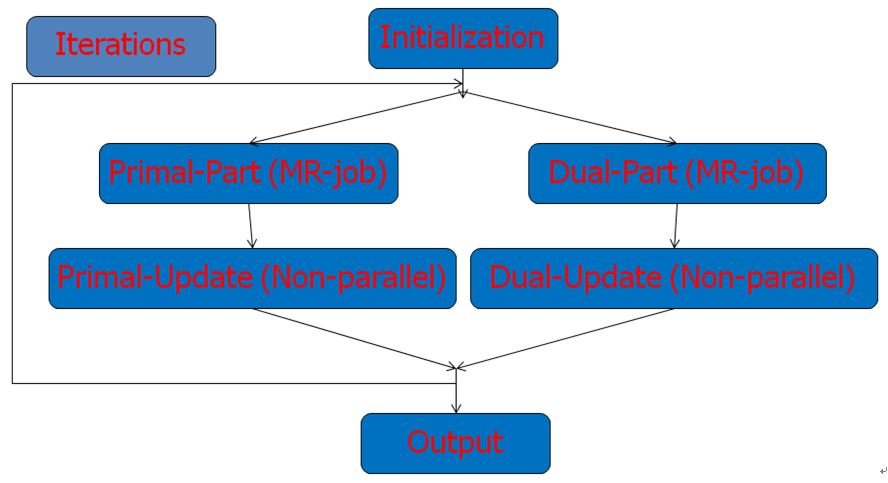
\includegraphics[height=3.5cm,width=6cm]{img/framework.png}
\caption{Parallel implementation flow chart for PSUBPLR-MR}
\end{figure}

For the parallelization period in the \textit{primal mapreduce job}, we take advantage of the MapReduce design that takes in every data instance in the training matrix.
Instead of the fashion in the sequential algorithm that we only sample a data instance in the primal update step, we compute gradients from "almost" all data instances and make the weighted average value according to vector $\bp$ as the output gradient for update.
The details of this algorithm design is shown in \textbf{Procedure Primal-Map(inputfile)} and \textbf{Procedure Primal-Reduce(key in, value in)}.
Here, we employ a randomization when we compute those "almost" all gradients.
As you can interpret from line 7 and 8 from \textbf{Procedure Primal-Map(inputfile)}, if $r=0$, then all data instances are computed.
As the expectation value for $\bp_t(i_t)$ is $\frac{1}{n}$, we normally set $r$ to range from 0 to 1.
For the parallelization period in the \textit{dual mapreduce job}, we actually implement an embarrassingly parallel operation.
It simply computes an individual value for each data instance in a parallel mode. It does not even need a reduce session.

There are also three more things that have to be addressed here.
First is the parameter passing issues. It critical to choose an efficient way to pass the updated parameters between iteration and even between different MapReduce jobs.
It is even more challenging when we have to deal with HDFS. It is clear that the fastest communication way is to pass parameters by \textit{Configuration()}.
However, it always has memory buffer size limits, and will greatly impair scalability when the number of parameters is huge.
Another way is to compress the parameter sequence in a string when sending and uncompress them when receiving. It has computational overhead and it still can not avoid the issue of memory buffer limit. 
Thinking back on the philosophy of the design of Hadoop, the natural thing is to pass parameters by file, the same way to pass all the data.
We admit that it is inefficient, but it is the only way to support for large datasets.

The second issue is the small changes we make to cater for the $\ell_2$-penalty and $\ell_1$-penalty. The changes is only made in \textbf{Procedure PrimalUpdate}.
It does not affect little for the implementation, and the extension is just the same as that in \textbf{Algorithm SLLR}.
To have a brief and standard framework, we omit the explanation here.

The datasets are always sparse for PLR is when data dimensionally is high. This makes us focus on dealing with data sparsity issue when writing code.
This is the third important thing for the algorithm, though it reflects nowhere from the pseudo-code.
Instead of naively writing the simple code for data intensive situations, we assign the index value for each data value in the sparse vector, and all computations are changed accordingly.
This gives us great efficiency improvement, and all results in section~\ref{sec:experiment} are using the code for sparsity.

\subsection{Parallel Sublinear algorithms in Spark}
The algorithm to solve sublinear learning for penalized logistic regression in Spark is shown below.
In the pseudo-code of Algorithm 3, Procedure for PrimalUpdate and Procedure for Dual-Map are the same as those in \textbf{Algorithm  PSUBPLR-MR}.
    \begin{table}[ht]
	\begin{tabular}{l}
    \hline\noalign{\smallskip}
	\textbf{Algorithm 3} PSUBPLR-SPARK \\
	\noalign{\smallskip}
	\hline
	\noalign{\smallskip}
    1:  ~Input parameters: $\varepsilon, \nu~or~\gamma, X, Y, n, d$ \\
    2:	~Initialize parameters: $T, \eta, {\mathbf{u}}_{0}, {\bw}_{1}, {\mathbf{\bq}}_{1}, {b}_{1}$\\
    3:  ~points $\leftarrow$ spark.textFile(inputfile).map(parsePoint()).cache() \\
    4:  ~Iterations: $t=1 \sim T$ \\
    5:  ~\tspace gradient $\leftarrow$ points.map($(\frac{1}{1+e^{-y((\bw^T \textbf{x})+b)}}-1) * y * \bp [index]$).reduce( \_ + \_ ) \\
    6:  ~\tspace ($\bw_{t+1}, b_{t+1}$)$\leftarrow$PrimalUpdate($\bw_t, b_t$) \\
    7:  ~\tspace Choose $j_t \leftarrow j$ with probability ${{\bw}_{t+1}\lj}^{2}/{\|{\bw}_{t+1}\|_2}^{2} $ \\
    8:  ~\tspace pAdjust $\leftarrow$ points.map(MW-Update()).reduce(copy()) \\
    9:  ~\tspace $\bp_{t+1}$$\leftarrow$DualUpdate($\bp_t$)  \\
    10: \textbf{Output}($\bw, b$) \\
    \hline
    \end{tabular}
	\end{table}

This parallel design is very similar to that of \textbf{Algorithm  PSUBPLR-MR}.
The most important difference is the \textit{cache()} operation in line 3.
To make it work in Spark, we follow the rules to construct an RDD for each data instance.
Also to cater for data sparsity, the design is the every data value correspond to its individual index. And the index also participate in the computation along with the value.
We also omit the changes for $\ell_2$-penalty and $\ell_1$-penalty here to make the algorithm easier to be understood.

We can now study the running time of parallel sublinear method for PLR.
In parallel mode, the primal update contains an update of $w_t$, which takes $O(n)$ time.
And the dual update contains a $\ell_2$-sampling process for the choice of $j_t$ in $O(d)$ time, and an update of $\bp$ in $O(1) time$.
Altogether, each iteration takes $O(n+d)$ time, which is sublinear to the dataset size.
Compared to the analysis of sequential algorithm, parallelization does not change computational complexity.
However, by reducing the constant coefficient from 2 to 1 in each iteration, it can be two times faster than sequential sublinear algorithm theoretically.
Moreover, by starting two separate MapReduce jobs in a iteration simultaneously, the running time can be reduced to $O(max\{n,d\})$.

\subsection{Parallel Gradient Descent in Spark}
The parallel gradient descent method to solve PLR in Spark is shown below.
    \begin{table}[ht]
	\begin{tabular}{l}
    \hline\noalign{\smallskip}
	\textbf{Algorithm 4} PGDPLR-SPARK \\
	\noalign{\smallskip}
	\hline
	\noalign{\smallskip}
    1:  Input parameters: $\varepsilon, \nu~or~\gamma, X, Y, n, d$ \\
    2:	Initialize parameters: $T, \eta, {\mathbf{u}}_{0}, {\bw}_{1}, {\mathbf{\bq}}_{1}, {b}_{1}$\\
    3:  points $\leftarrow$ spark.textFile(inputfile).map(parsePoint()).cache() \\
    4:  Iterations: $t=1 \sim T$ \\
    5:  \tspace gradient $\leftarrow$ points.map($(\frac{1}{1+e^{-y((\bw^T \textbf{x})+b)}}-1) * y * \bp [index]$).reduce( \_ + \_ ) \\
    6:  \tspace $\bw_{t+1} = \bw_t - gradient * \textbf{x}$ \\
    7:  \tspace $b = b - gradient$ \\
    8:  \textbf{Output}($\bw, b$) \\
    \hline
    \end{tabular}
	\end{table}

In the pseudo-code of Algorithm 4, we can find that it is implemented in an embarrassingly parallel mode.
We can take in all the data at the same iteration and just compute the gradient in a MapReduce fashion.
As for the \textit{cache()} operation and RDD design for data sparsity, it is the same as \textbf{Algorithm PSUBPLR-SPARK}.

\subsection{Online Stochastic Gradient Descent in Mahout}
Though SGD is an inherently sequential algorithm, it is blazingly fast and thus it is not a problem for Mahout's implementation to handle training sets of tens of millions of examples.
With the down-sampling typical in many datasets, this is equivalent to a dataset with billions of raw training examples.
The SGD system in Mahout is an online learning algorithm which means that you can learn models in an incremental fashion and that we can do performance testing as your system runs.
This also means that we can stop training when a model reaches a target level of performance.
The SGD framework includes classes to do online evaluation using cross validation (the \textit{CrossFoldLearner}) and an evolutionary system to do learning hyper-parameter optimization on the fly (the \textit{AdaptiveLogisticRegression}).
The \textit{AdaptiveLogisticRegression} system makes heavy use of threads to increase machine utilization.
The way it works is that it runs 20 \textit{CrossFoldLearners} in separate threads, each with slightly different learning parameters.
As better settings are found, these new settings are propagating to the other learners.

Because the SGD algorithms need to have fixed length feature vectors and because it is a pain to build a dictionary ahead of time, most SGD applications use the hashed feature vector encoding system that is rooted at \textit{FeatureVectorEncoder}.
The basic idea is that you create a vector, typically a \textit{RandomAccessSparseVector}, and then you use various feature encoders to progressively add features to that vector.
The size of the vector should be large enough to avoid feature collisions as features are hashed.
There are specialized encoders for a variety of data types.
You can normally encode either a string representation of the value you want to encode or you can encode a byte level representation to avoid string conversion.
In the case of \textit{ContinuousValueEncoder} and \textit{ConstantValueEncoder}, it is also possible to encode a null value and pass the real value in as a weight.

In our implementation, we use \textit{RandomAccessSparseVector} for data sparsity and the function call by \textit{OnlineLogisticRegression} to train.
We also do the cross validation part. However, to be synchronized with other methods, we write our own code to do cross validation.
	
\section{Experiments} \label{sec:experiment}
In this section, we conduct an empirical analysis of our algorithms.

We choose five open datasets to run all six test programs:	
The	Simulated \textbf{2d} dataset has 2 features and 200 instances.
The	\textbf{20NewsGroup} dataset has 16428 features and 1988 instances. We split it into a training set of 1800 instances and a test set of 188 instances.	
The	third test dataset is the \textbf{Gisette}~\cite{guyon2004result} dataset, which has 5000 features and 7000 instances. We split it into a training set of 6000 instances and a test set of 1000 instances.
The	fourth test dataset is the \textbf{ECUESpam}~\cite{DelanyKBS05} dataset, which has 100249 features and 10678 instances (after proper preprocessing). We split it into a training set of 9000 instances and a test set of 1687 instances.
Finally, we have the \textbf{URL-Reputation}~\cite{ma2009identifying} dataset, which has 3231961 features and 2376130 instances.
We split it into a training set of 2356130 instances and a test set of 20000 instances.
Apart from the Simulated \textbf{2d} dataset, other four datasets are all sparse. Details are shown in Table~\ref{tab:table1}.
We randomly repeat such split 20 times and our analysis is based on the average performance of 20 repetitions.

%Particularly, we illustrate test errors in terms of accuracy and convergence in terms of MAP, both with respect to running time.

\begin{table}[h]
\centering
\caption{Datasets}\label{tab:table1}
\begin{tabular}{|c|c|c|c|c|c|}
\hline
    Name           & \# of Feat. & \# of Inst. & Sparsity & \# of Nonzeros & \# of +1 Inst. / \# of -1 Inst.\\
\hline
    2d             & 2             & 200            & 1.0                  & 400                 & 1.000 \\
\hline
    20NewsGroup    & 16428         & 1988           & $7.384\times10^{-3}$ & 238511              & 1.006 \\
\hline
    Gisette        & 5000          & 7000           & 0.12998              & 4549319             & 1.000 \\
\hline
    ECUESpam       & 100249        & 10687          & $2.563\times10^{-3}$ & 2746159             & 5.882 \\
\hline
    URL-Reputation & 3231961       & 2376130        & $3.608\times10^{-35}$ & 277058644           & 0.500 \\
\hline
\end{tabular}
\end{table}

The cluster that we implement on has the following configurations shown in Table~\ref{tab:table2}.
\begin{table}[h]
\centering
\caption{Cluster Information}\label{tab:table2}
\begin{tabular}{|c|c|}
\hline
    CPU Model & Intel Xeon E5-1410: 2.80GHz \\
\hline
    Number of node & 6 \\
\hline
    Number of CPU per node & 4 Cores, 8 Threads \\
\hline
    RAM per node & 16G \\
\hline
    Disk per node & 4T HDD\\
\hline
    Interconnection Method & Gigabyte Ethernet  \\
\hline
\end{tabular}
\end{table}

2d-dataset (separation graph)
\begin{figure}[tb] \label{fig:02}
\center 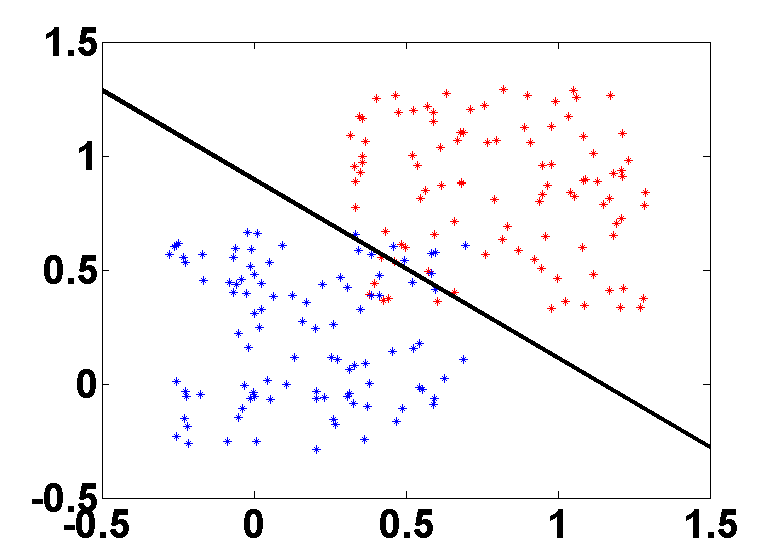
\includegraphics[height=5cm,width=7cm]{img/show-2d.png}
\caption{2d Dataset, Visual Result}
\end{figure}


\begin{figure}[tb] \label{fig:03}
\center 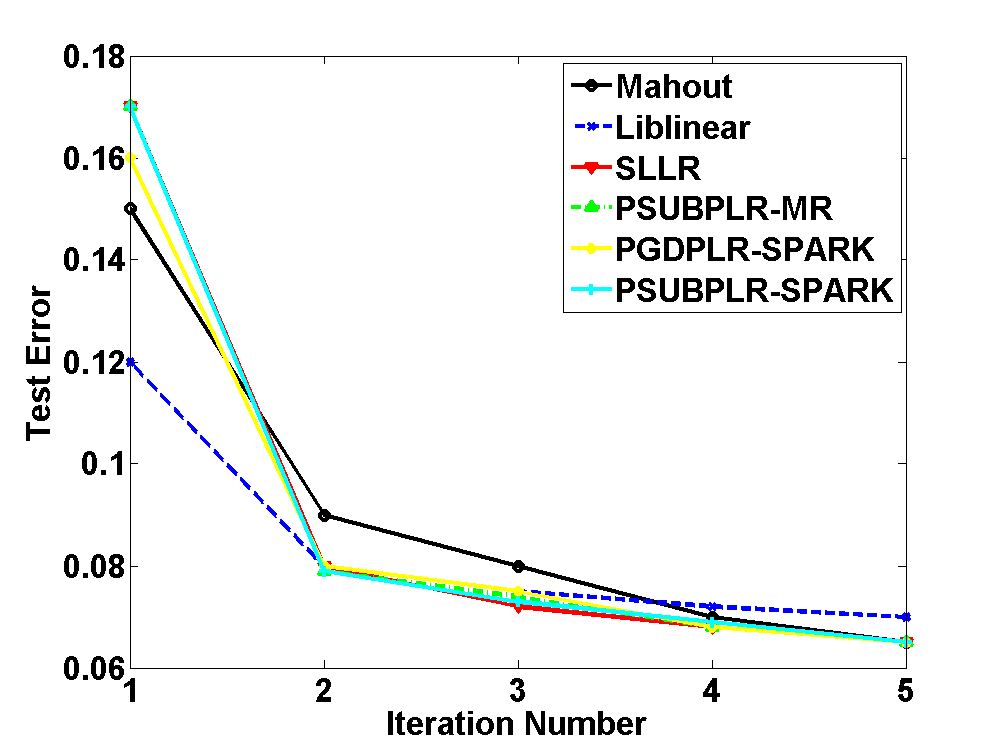
\includegraphics[height=4.5cm,width=6cm]{img/2d_accuracy_iteration.png}
\caption{2d Dataset, Visual Result}
\end{figure}

\begin{figure}[tb] \label{fig:04}
\center 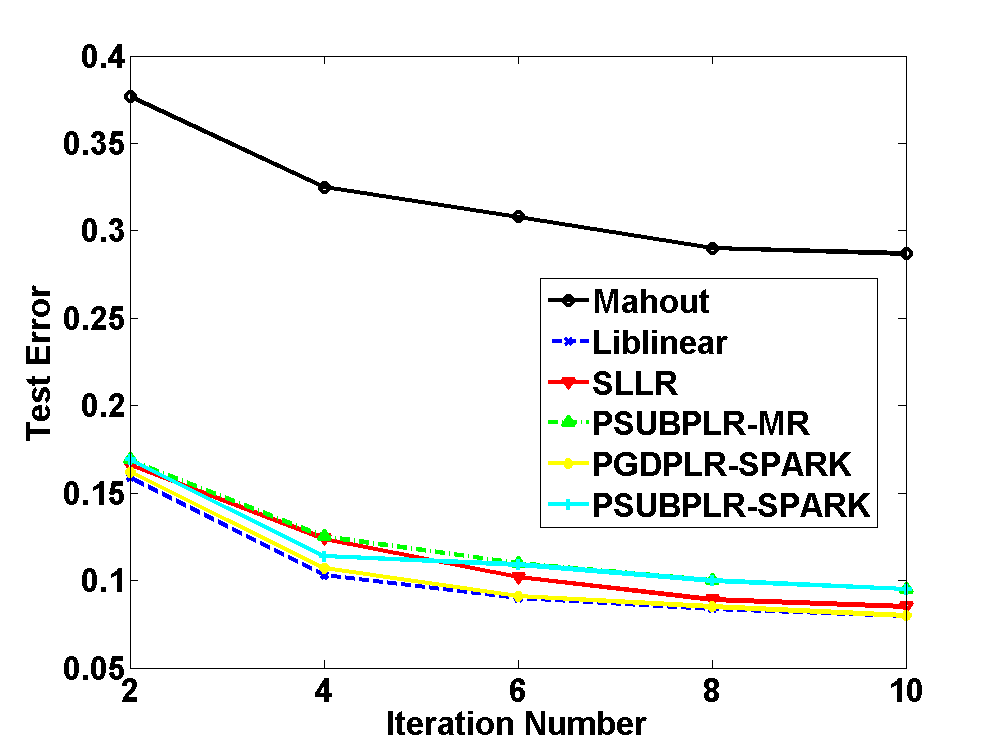
\includegraphics[height=4.5cm,width=6cm]{img/20NewsGroup_accuracy_iteration.png}
\caption{2d Dataset, Visual Result}
\end{figure}

\begin{figure}[tb] \label{fig:05}
\center 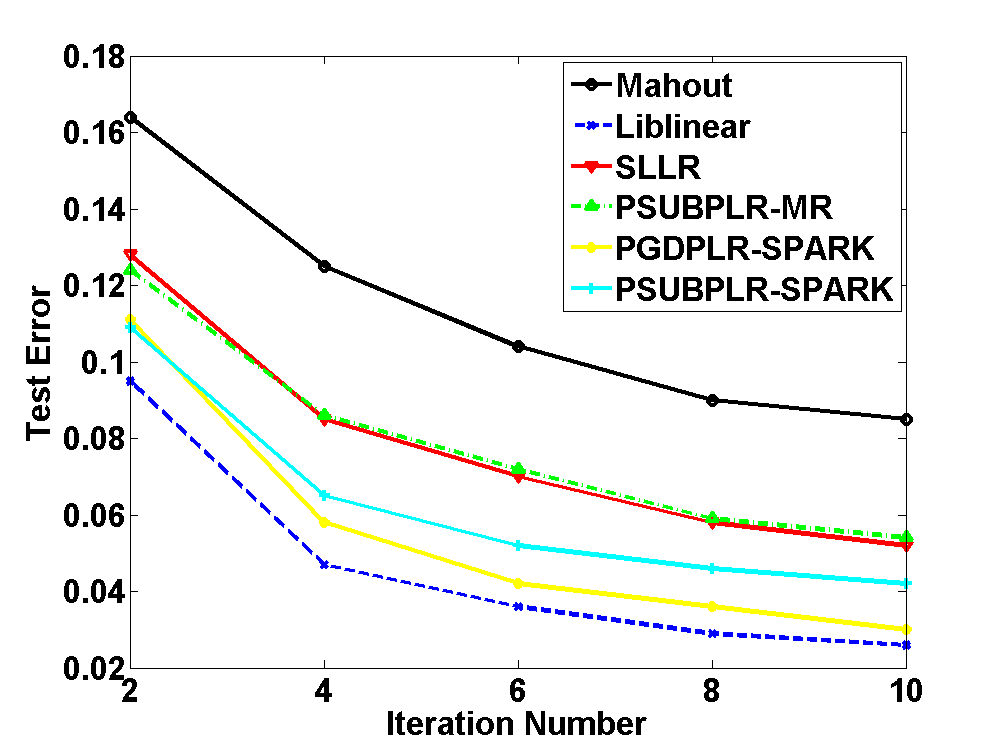
\includegraphics[height=4.5cm,width=6cm]{img/Gisette_accuracy_iteration.png}
\caption{2d Dataset, Visual Result}
\end{figure}

\begin{figure}[tb] \label{fig:6}
\center 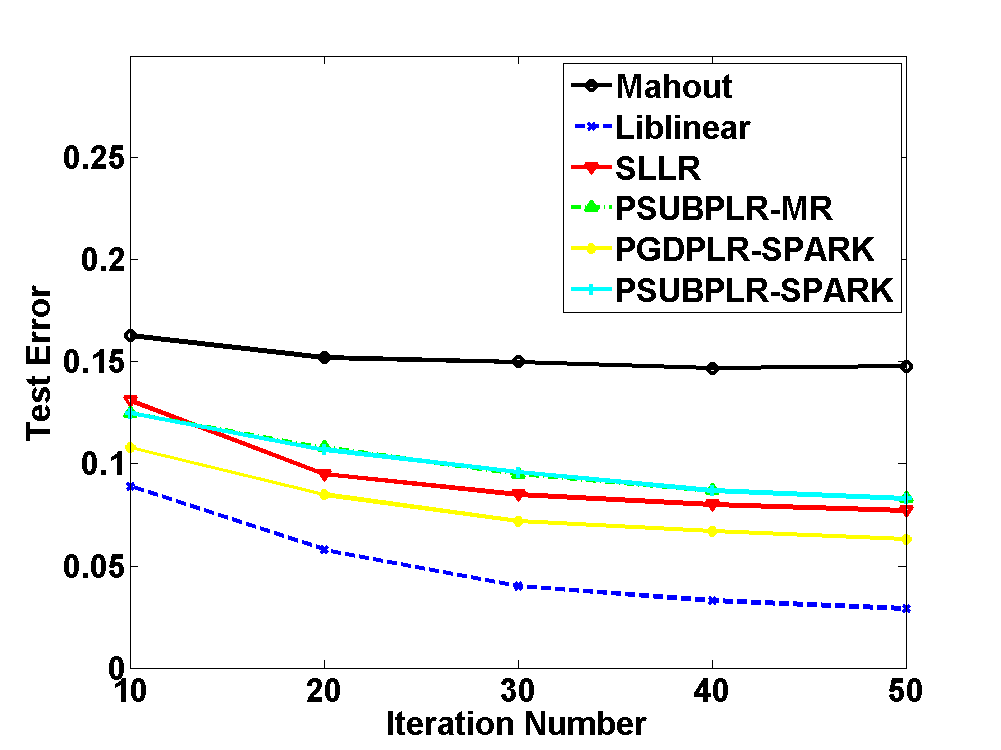
\includegraphics[height=4.5cm,width=6cm]{img/ECUESpam_accuracy_iteration.png}
\caption{2d Dataset, Visual Result}
\end{figure}

\begin{figure}[tb] \label{fig:07}
\center 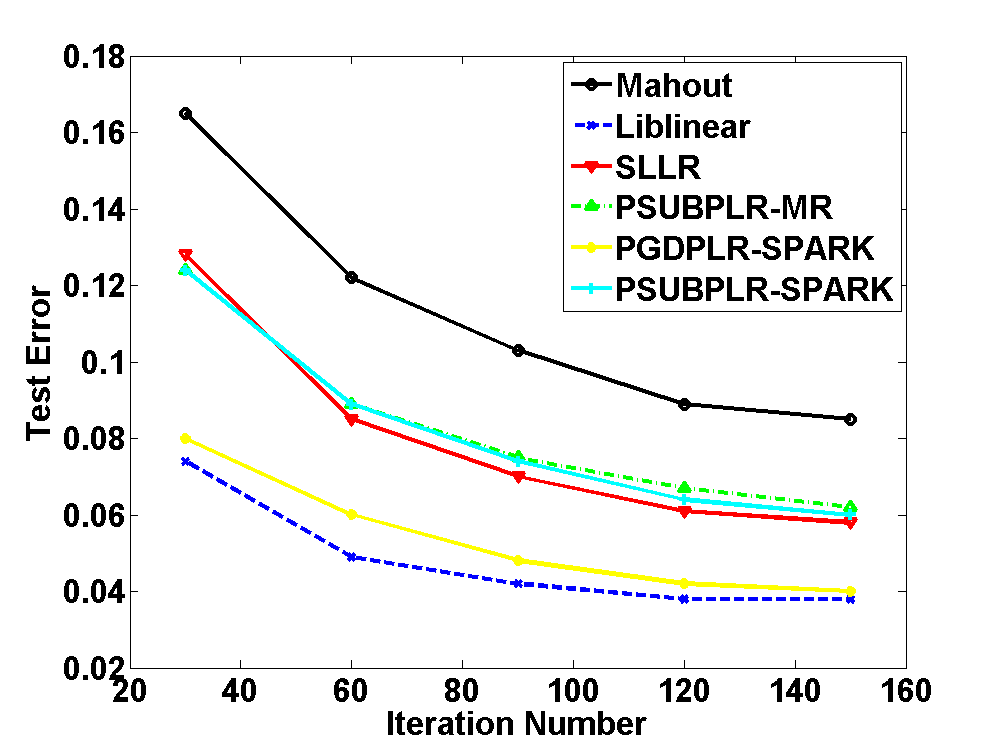
\includegraphics[height=4.5cm,width=6cm]{img/URL-Reputation_accuracy_iteration.png}
\caption{2d Dataset, Visual Result}
\end{figure}


\begin{figure}[tb] \label{fig:08}
\center 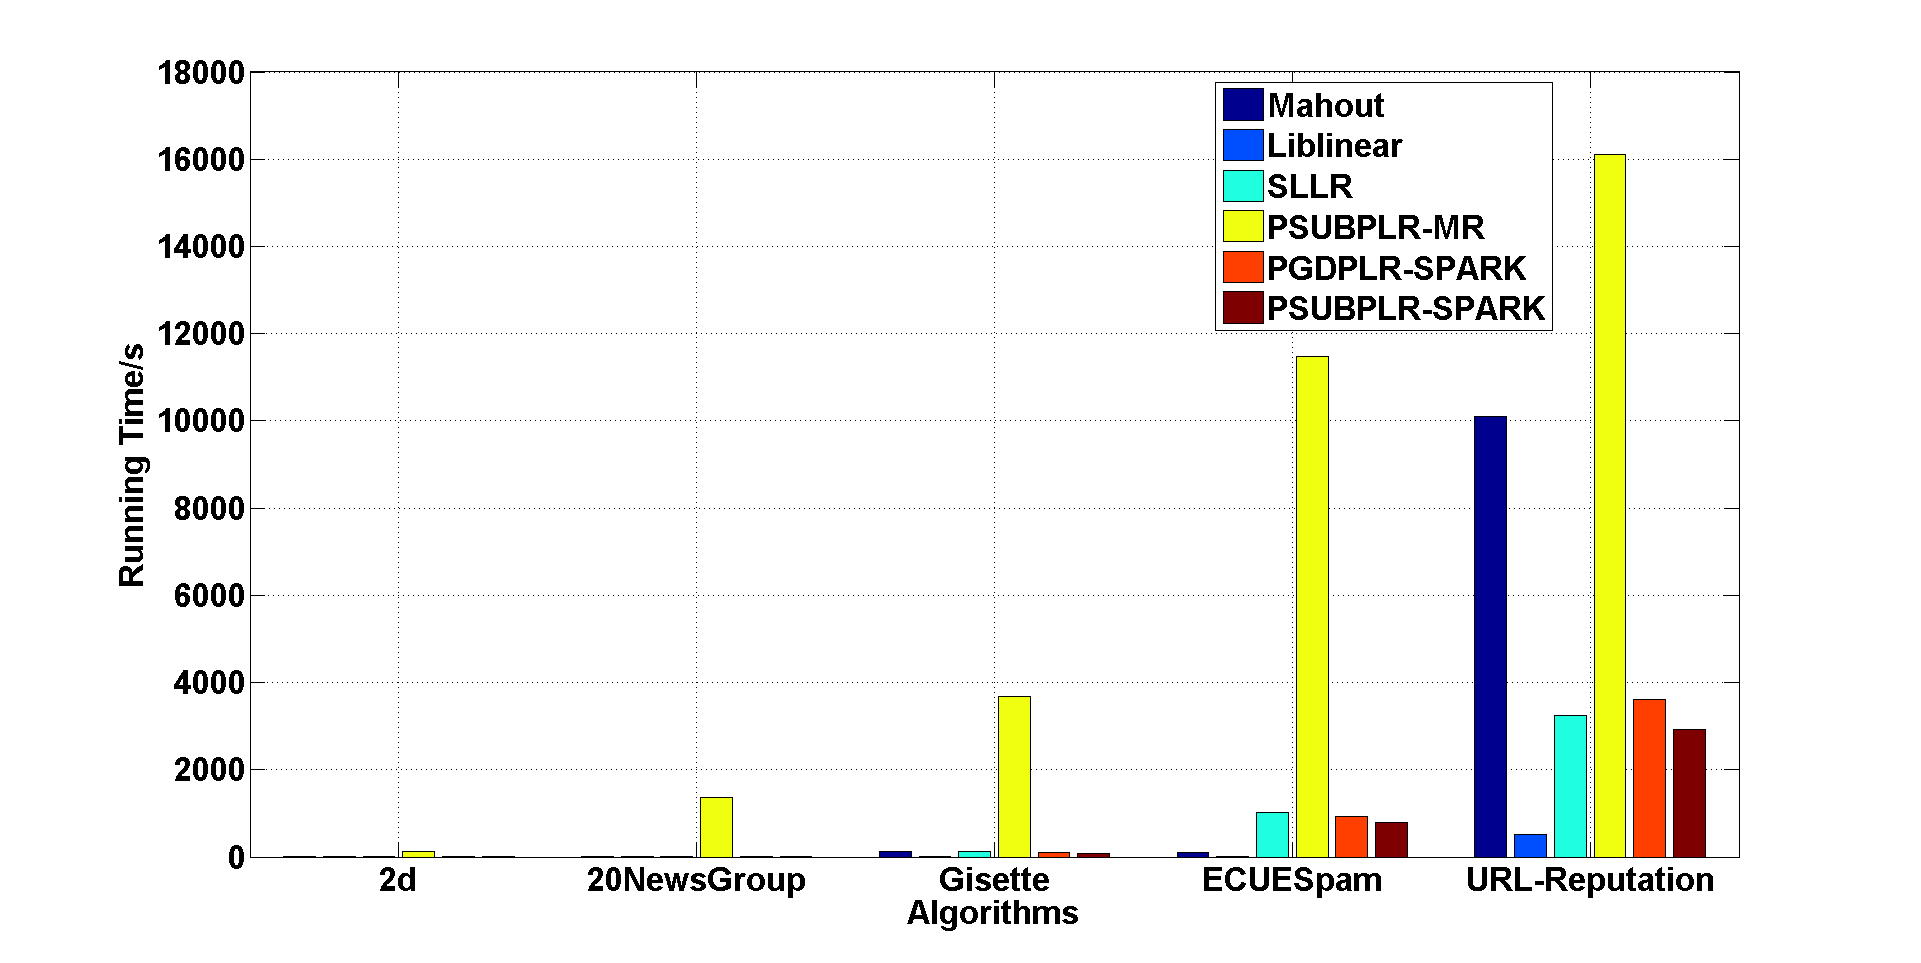
\includegraphics[height=5cm,width=10cm]{img/all_time.png}
\caption{2d Dataset, Visual Result}
\end{figure}


\begin{figure}[tb] \label{fig:09}
\center 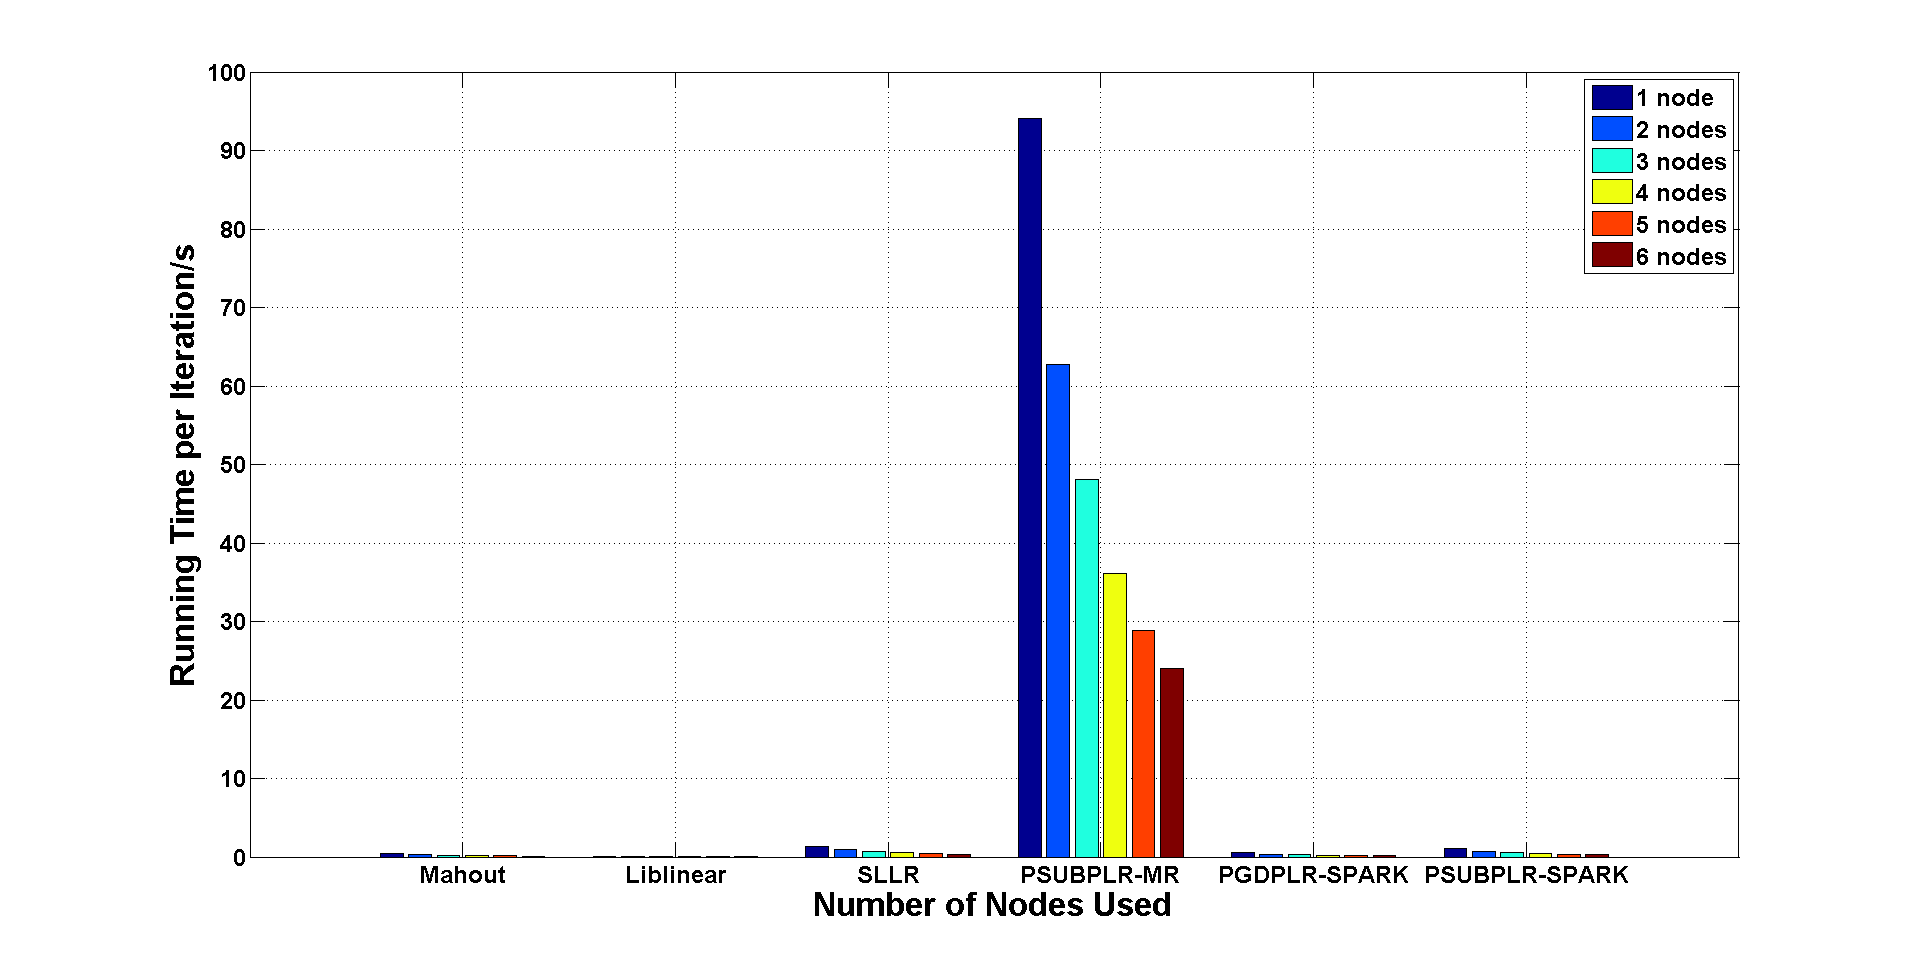
\includegraphics[height=5cm,width=10cm]{img/2d_time.png}
\caption{2d Dataset, Visual Result}
\end{figure}

\begin{figure}[tb] \label{fig:10}
\center 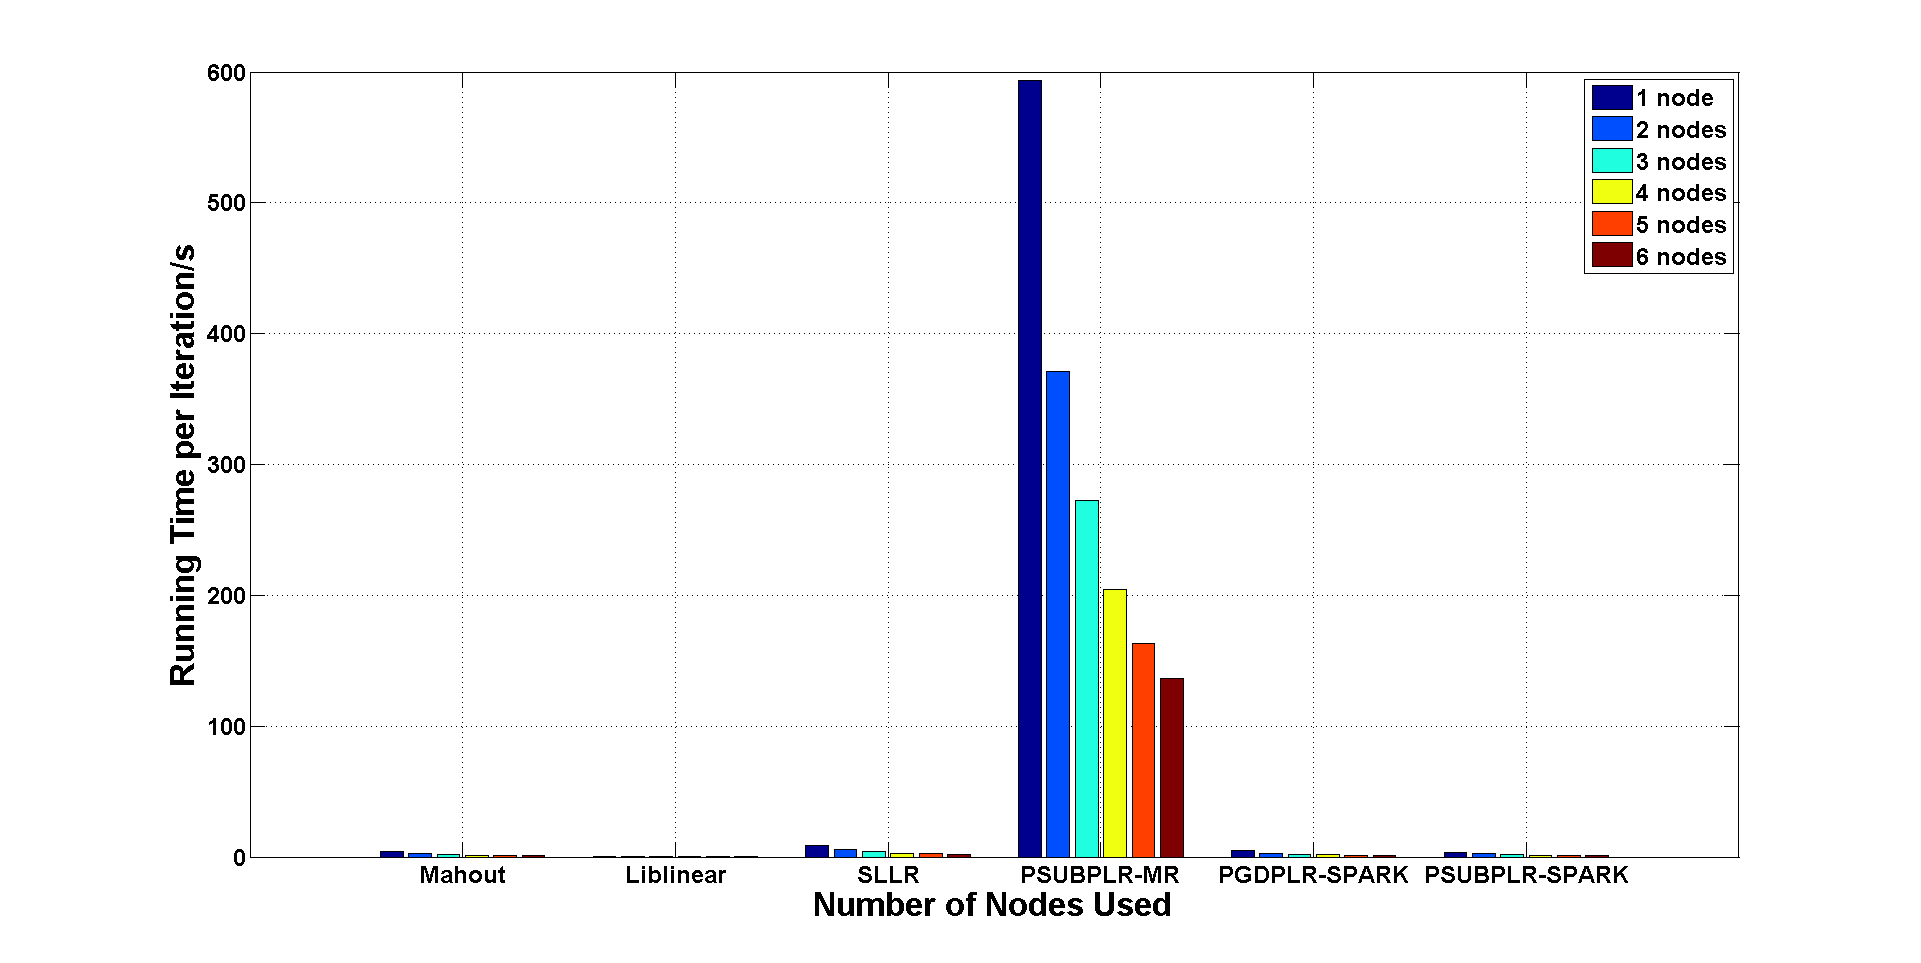
\includegraphics[height=5cm,width=10cm]{img/20NewsGroup_time.png}
\caption{2d Dataset, Visual Result}
\end{figure}

\begin{figure}[tb] \label{fig:11}
\center 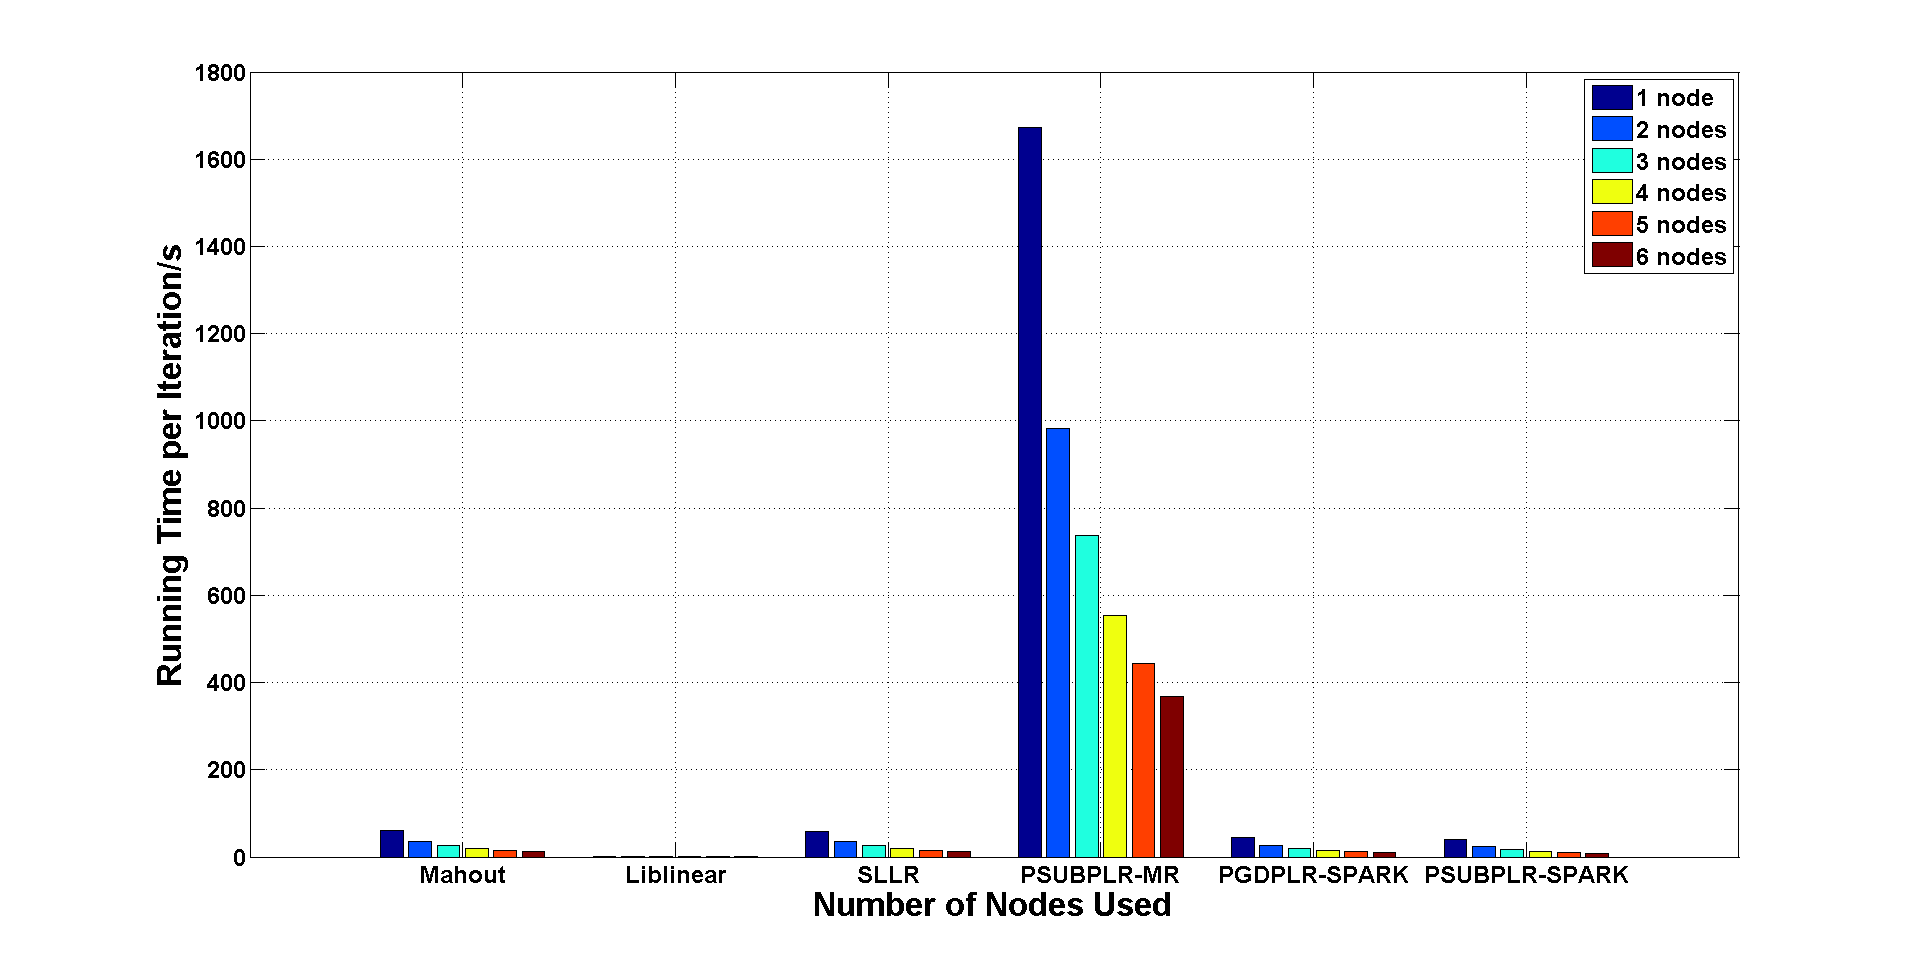
\includegraphics[height=5cm,width=10cm]{img/Gisette_time.png}
\caption{2d Dataset, Visual Result}
\end{figure}

\begin{figure}[tb] \label{fig:12}
\center 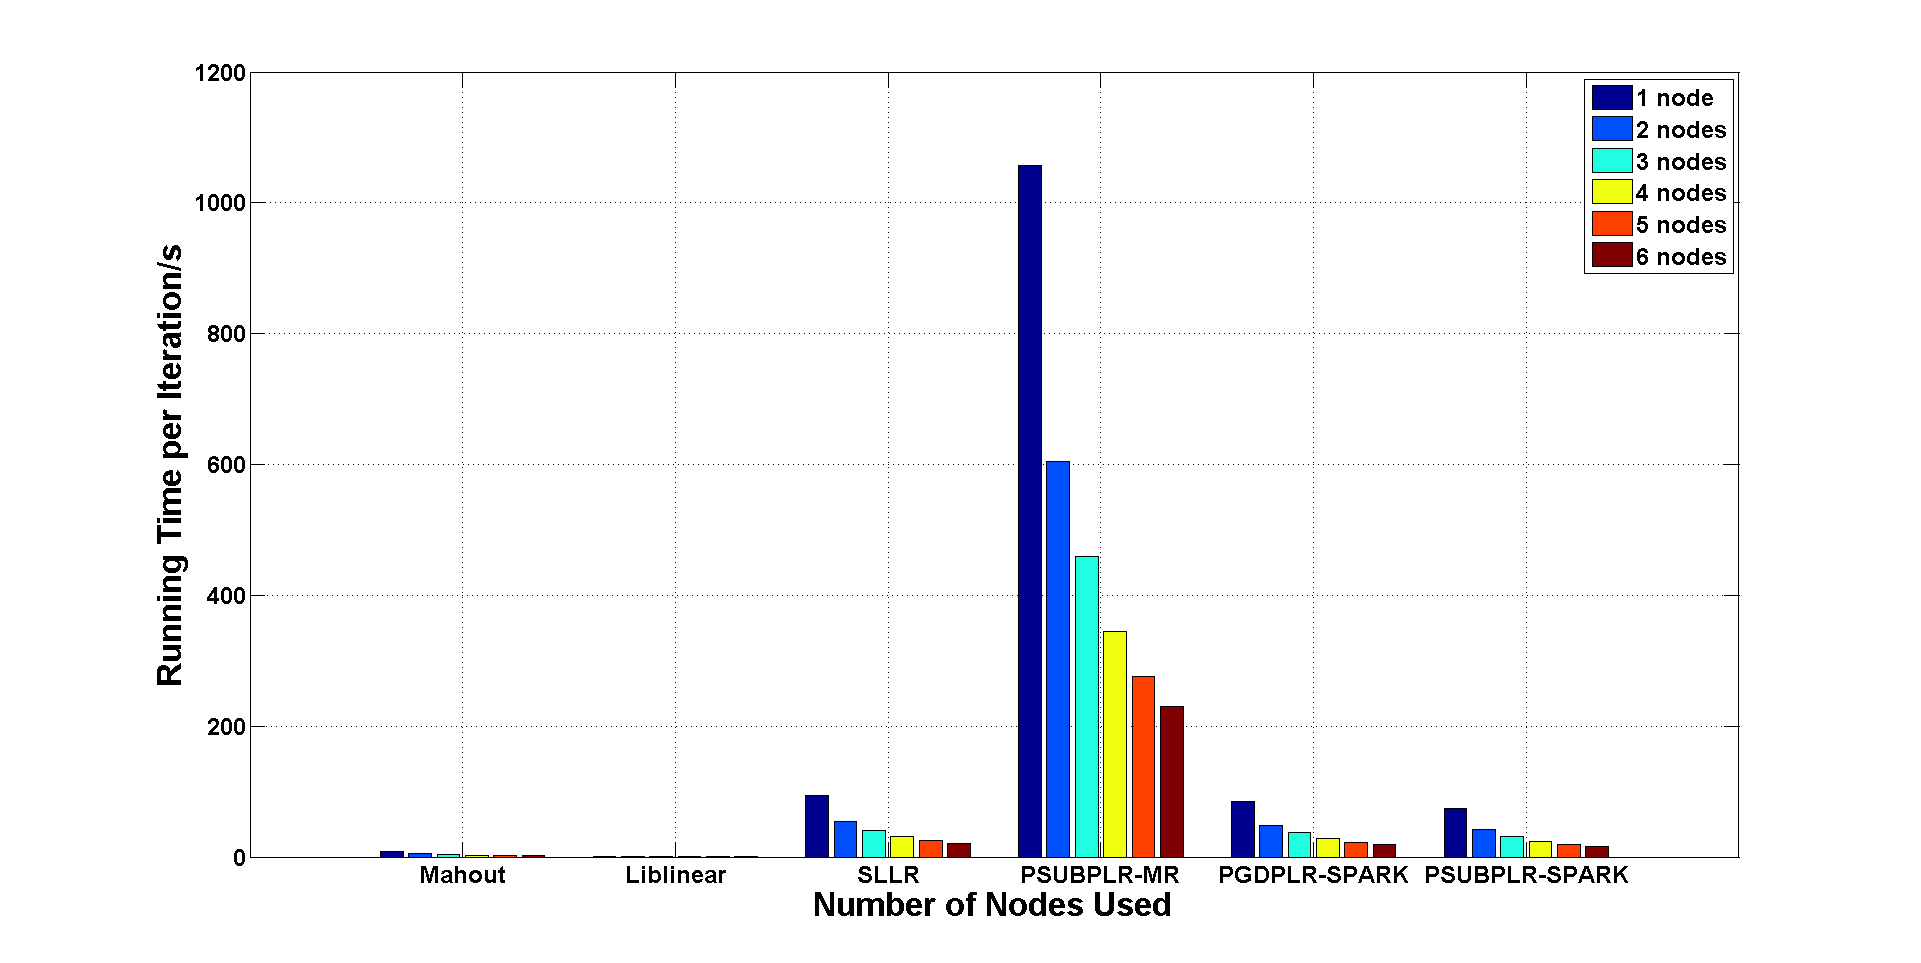
\includegraphics[height=5cm,width=10cm]{img/ECUESpam_time.png}
\caption{2d Dataset, Visual Result}
\end{figure}

\begin{figure}[tb] \label{fig:13}
\center 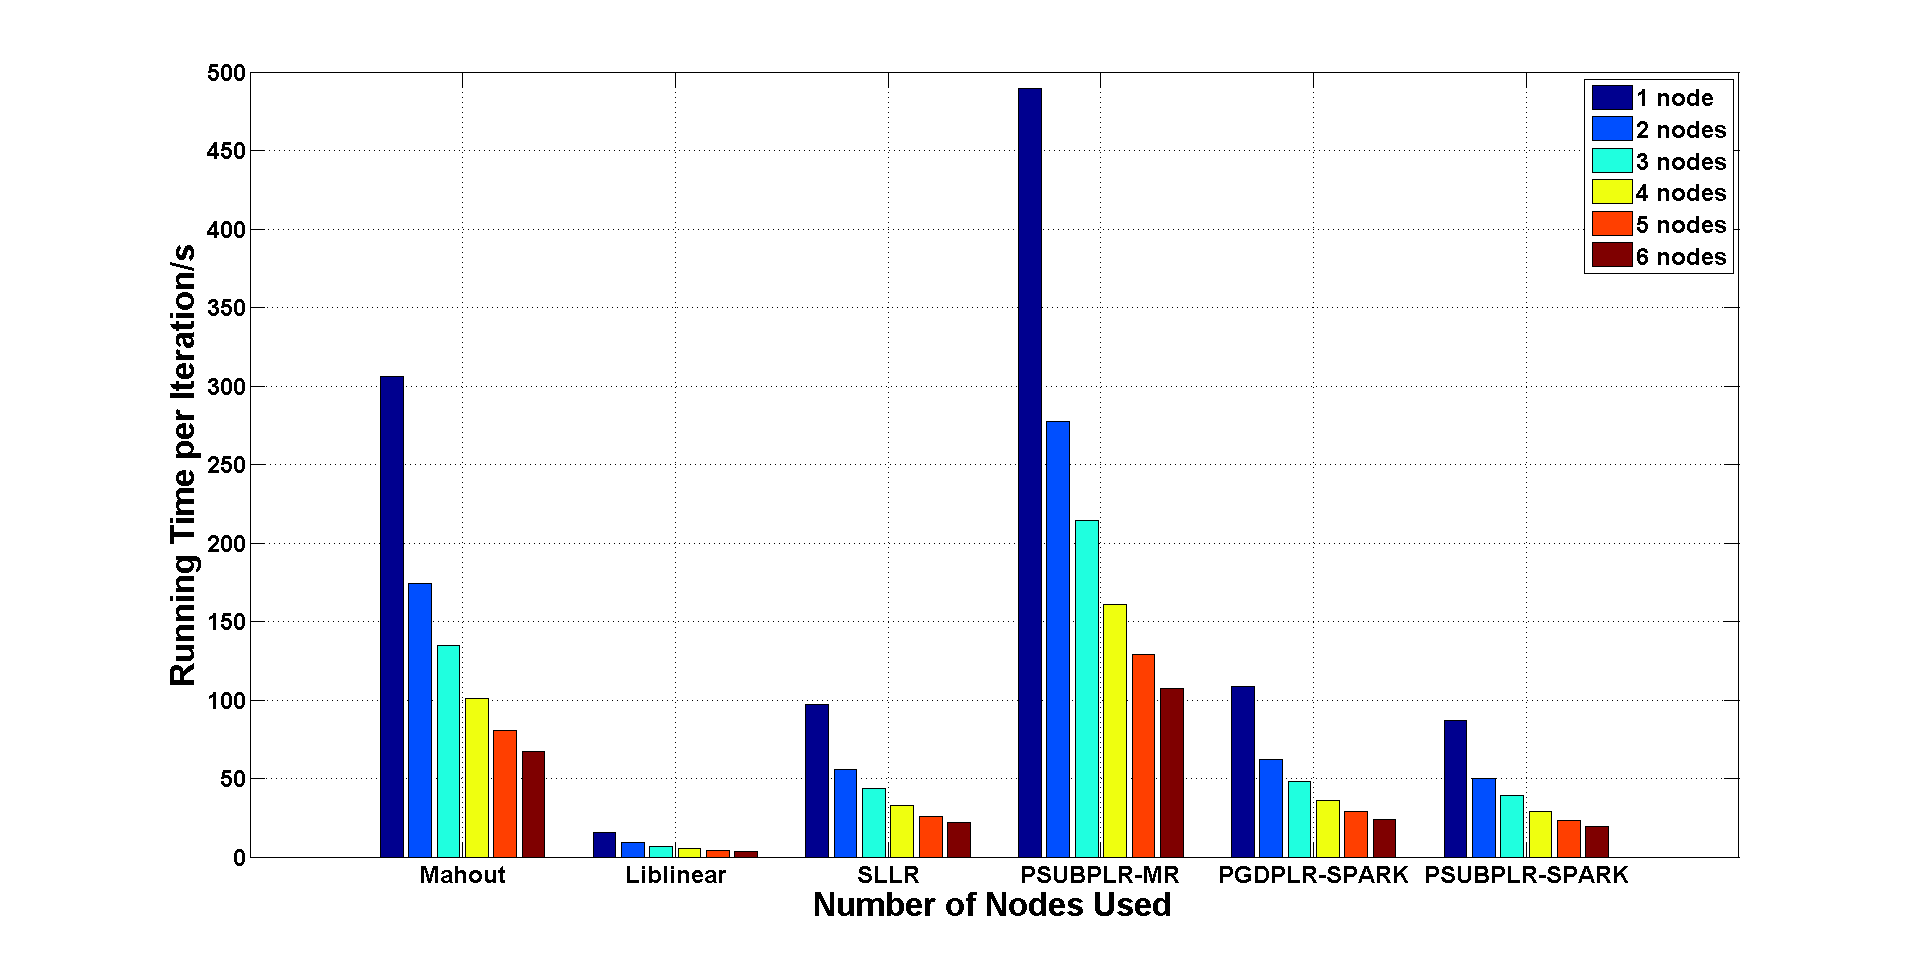
\includegraphics[height=5cm,width=10cm]{img/URL-Reputation_time.png}
\caption{2d Dataset, Visual Result}
\end{figure}


\begin{figure}[tb] \label{fig:14}
\center 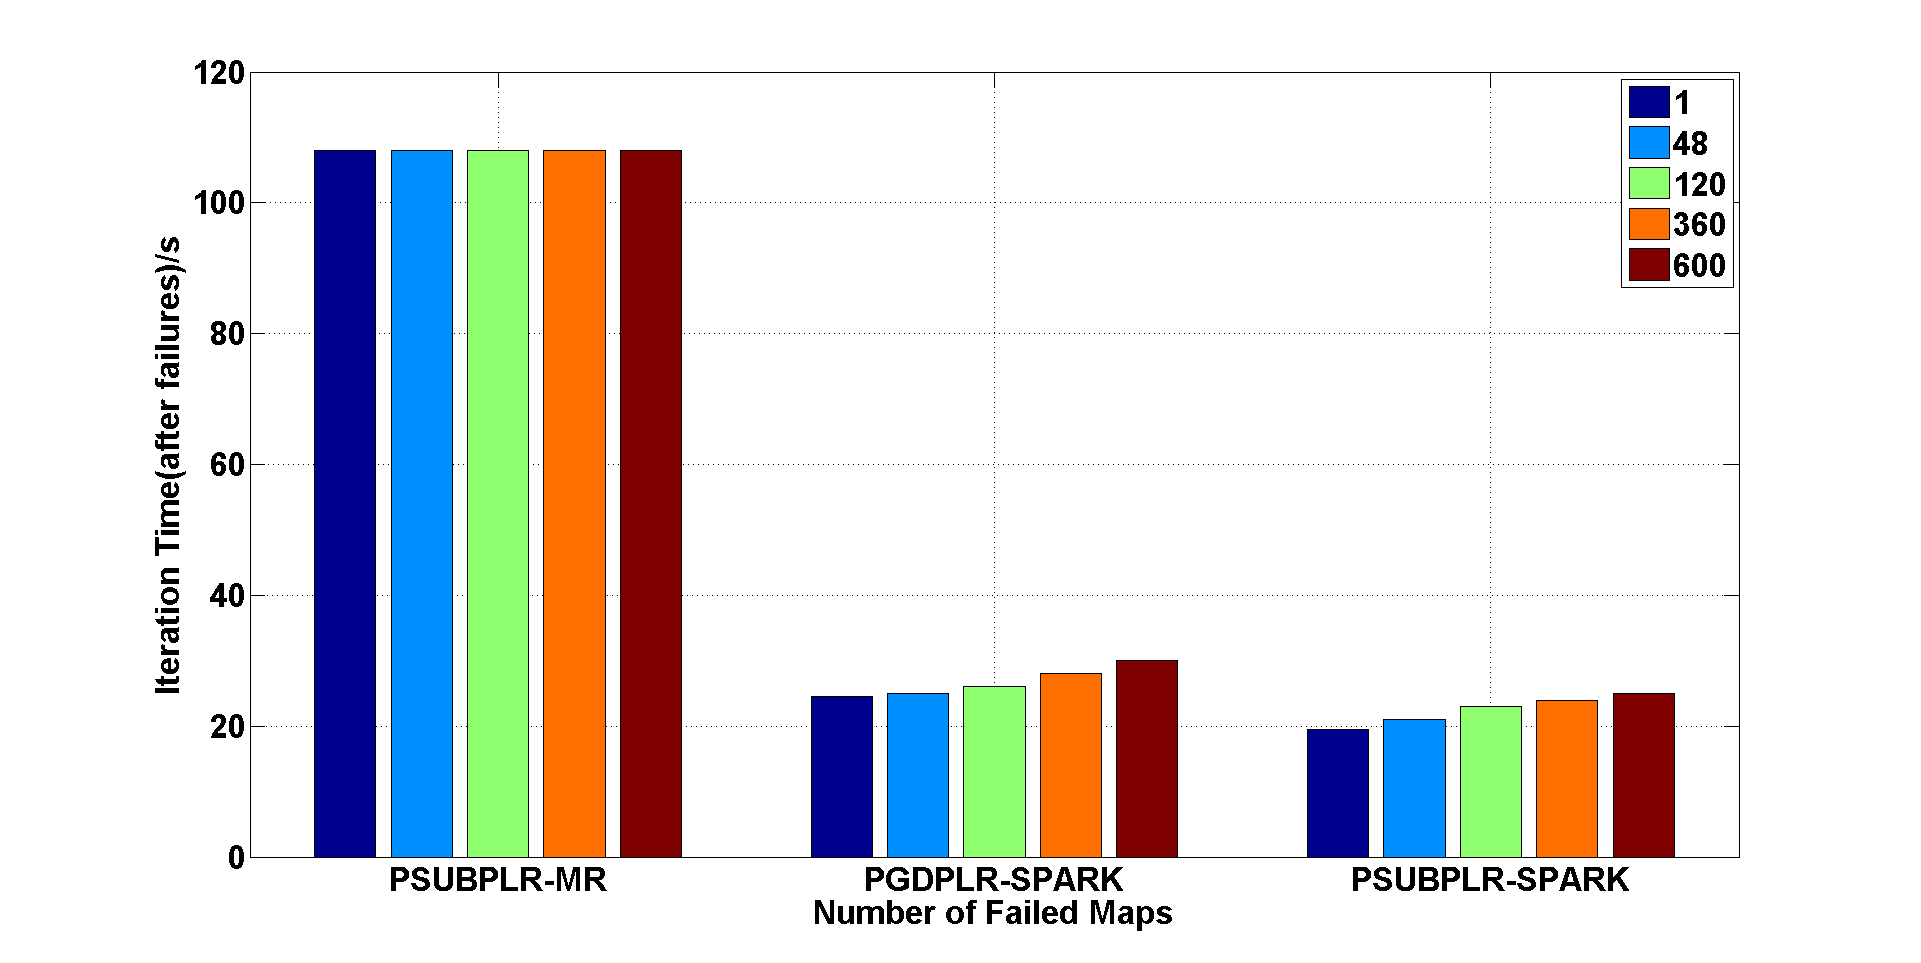
\includegraphics[height=5cm,width=10cm]{img/fault_tolerance.png}
\caption{2d Dataset, Visual Result}
\end{figure}

\comment{1: add 5 line graphs;one dataset each;x:iteration number;y:accuracy;6 lines}

\comment{2: add 1 bar graphs;x:different algorithms;y:time;one dataset as a group}

%\comment{3: add 5 line graphs;one dataset each;x:iteration number;y:MAP;6 lines}

\comment{4: add 5 bar graph;one dataset each;x:number of node used;y:time per iteration;each algorithm as a group}

\comment{5: Fault tolerance-add 1 bar graph;x:number of maps failed;y:time of the iteration;each algorithm as a group}

\comment{further parallelization in PSUBPLR-MR, Primal Map is the bottleneck}
\comment{parameter passing issues in PSUBPLR-MR, the effect in small dataset}
\comment{MR job start time}
\comment{baseline liblinear}
\comment{2d test method}
\comment{not all converge at the iteration shown}
\comment{symbol review}
\comment{single reducer of spark}
\comment{Iteration Number for SLLR explain}
\comment{Liblinear Url result}
\comment{fault tolerance: on url dataset,6 nodes}
Analysis points:

1: liblinear always performs the best; It fully utilizes memory; Single machine does not require communication; Disadvantage: cannot run large datasets, eg. ...(detailed statistics)

2: Mahout precision not good; especially for those positive and negative instances are not balanced datasets perform poorly; sequential algorithm that can run large data in an acceptable time; Advantage: running memory is low, scalability is good

3: Sublinear methods' accuracy is acceptable.; Parallel-sublinear has a small drop in precision.

4: Hadoop's big drawback: Most current cluster programming models are based on acyclic data flow from stable storage to stable storage. Benefits of data flow: runtime can decide where to run tasks and can automatically recover from failures. But acyclic data flow is inefficient. eg. ... (detailed statistics)

5: Spark's in memory strategy; not to use hdfs file; system maybe even improved

6: fast convergent

7: In general, different algorithms for different datasets and system requirement. For general purpose, we recommend subSpark.

\begin{table}[h]
\centering
\caption{Accuracy Result}\label{tab:table3}
\begin{tabular}{|c|c|c|c|c|c|}
\hline
           & 2d   & 20NewsGroup & Gisette & ECUESpam & URL-Reputation \\
\hline
Mahout     & 93.5\% & 71.3\% & 91.5\% & 85.2\% & 91.5\% \\
\hline
Liblinear  & 93.0\% & 92.0\% & 97.4\% & 97.1\% & $96.2\%^*$ \\
\hline
SLLR       & 93.5\% & 91.5\% & 94.8\% & 92.3\% & 94.2\% \\
\hline
PSUBPLR-MR & 93.5\% & 90.5\% & 94.6\% & 91.7\% & 93.8\% \\
\hline
PGDPLR-SPARK & 93.5\% & 92.0\% & 97.0\% & 93.7\% & 96.0\% \\
\hline
PSUBPLR-SPARK & 93.5\% & 90.5\% & 95.8\% & 91.7\% & 94.0\% \\
\hline
\end{tabular}
\end{table}

\begin{table}[h]
\centering
\caption{Running Time Result}\label{tab:table4}
\begin{tabular}{|c|c|c|c|c|c|}
\hline
           & 2d   & 20NewsGroup & Gisette & ECUESpam & URL-Reputation \\
\hline
Mahout     & 0.595s & 9.827s & 131.807s & 96.611s & 10100.209s \\
\hline
Liblinear  & 0.078s & 0.793s & 2.364s & 13.161s & $519.115s^*$ \\
\hline
SLLR       & 1.761s & 20.046s & 130.451s & 1028.185s & 3248.473s \\
\hline
PSUBPLR-MR & 120.186s & 1360.854s & 3687.941s & 11478.706s & 16098.260s \\
\hline
PGDPLR-SPARK & 0.681s & 10.517s & 99.156s & 924.020s & 3615.780s \\
\hline
PSUBPLR-SPARK & 1.325s & 8.571s & 89.094s & 796.802s & 2918.470s \\
\hline
\end{tabular}
\end{table}

\begin{table}[h]
\centering
\caption{Fault Tolerance}\label{tab:table5}
\begin{tabular}{|c|c|c|}
\hline
           & System Level & Algorithm Level \\
\hline
Mahout     & \Checkmark & \XSolid  \\
\hline
Liblinear  & \XSolid & \XSolid \\
\hline
SLLR  & \XSolid & \Checkmark \\
\hline
PSUBPLR-MR & \Checkmark & \Checkmark \\
\hline
PGDPLR-SPARK & \Checkmark & \XSolid \\
\hline
PSUBPLR-SPARK & \Checkmark &  \Checkmark \\
\hline
\end{tabular}
\end{table}

\comment{Will add explanation for table 5 later in next version of draft}

%Current URL-reputation Dataset Status
%\begin{figure}[tb] \label{fig:01}
%\center 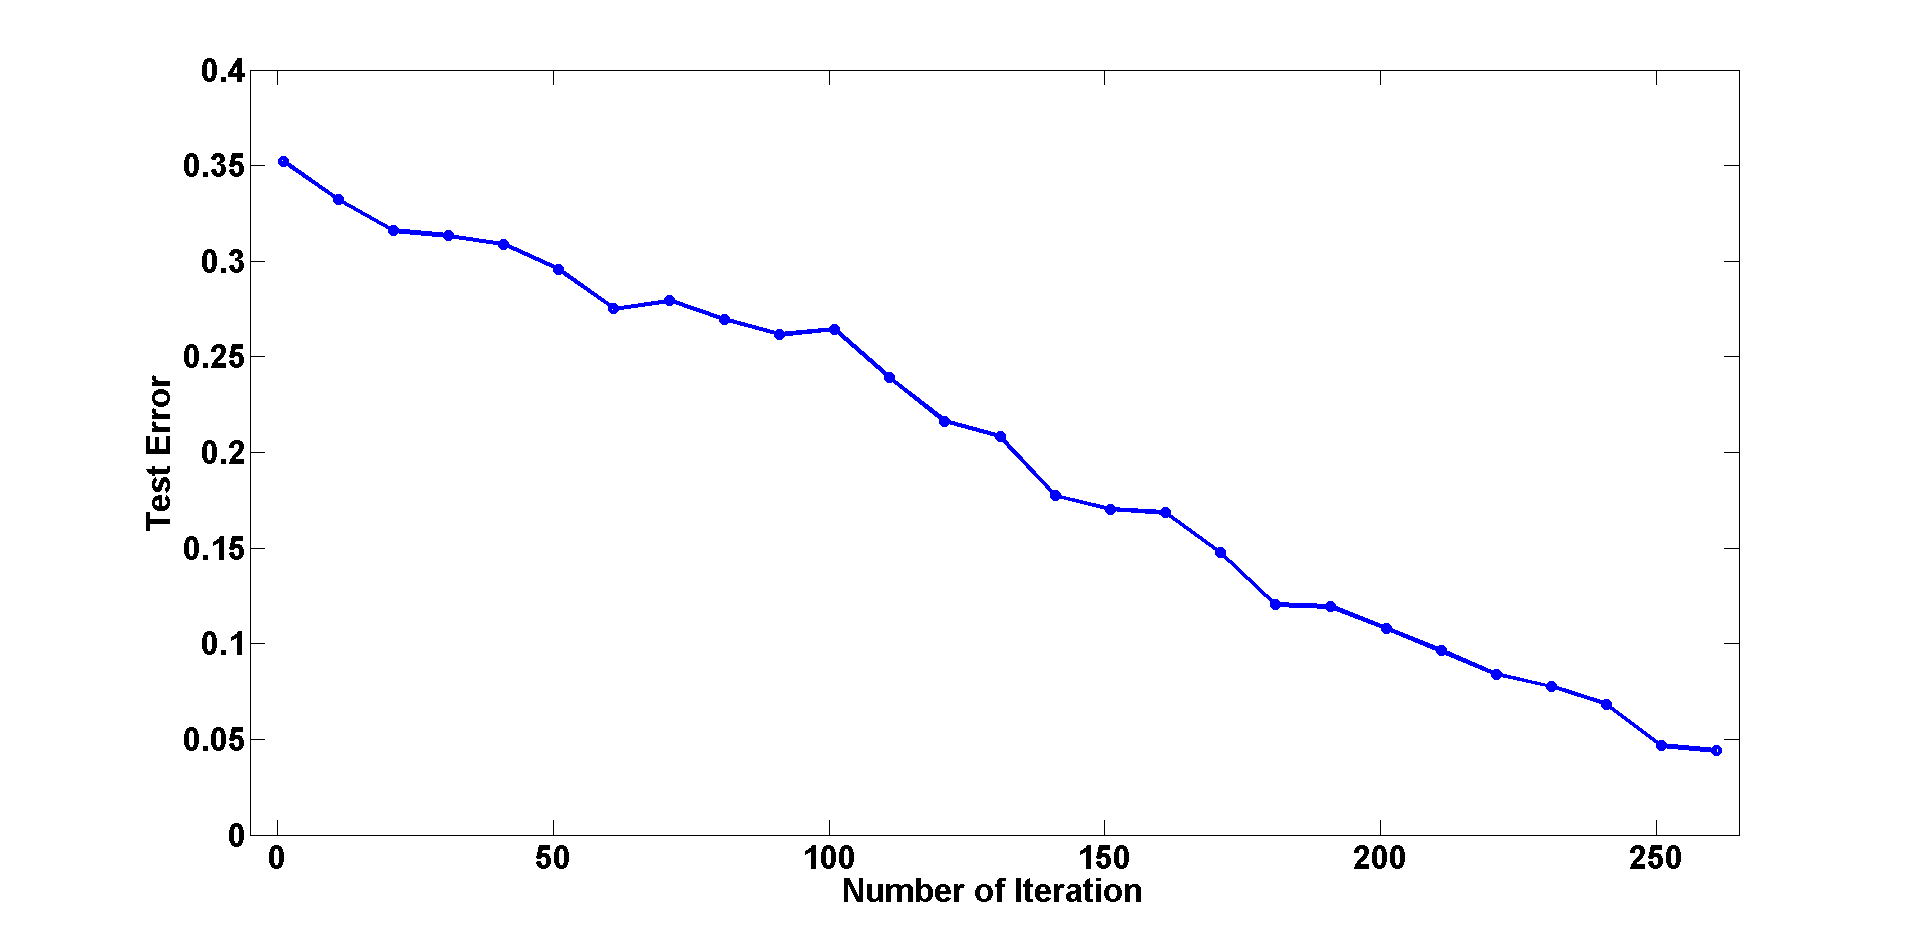
\includegraphics[height=5cm,width=10cm]{show1.png}
%\caption{URL-reputation Dataset, Performance Result}
%\end{figure}



\section{Conclusion} \label{sec:concl}
%conclusion & contribution & future work
In this paper we analyzed three approaches along with three systems to fitting PLR models for large-volume, high-dimensional data for classification.
The dataset size ranges from KB to GB.
Hadoop, Mahout and Spark are existing well-known parallel frameworks that can be implemented with large scale machine learning algorithms.
Parallel gradient Descent stochastic gradient descent are two existing state-of-art algorithms for parameter optimization in PLR.
We also present a novel parallel sublinear method and make a comparison between these algorithms implemented on different systems.
As the outcome shows, we claim parallel sublinear method implemented on Spark is the most computational efficient way to solve PLR for general purpose.
Moreover, fault tolerance can be provided for those lengthy distributed computations both on algorithm level and system level.
We discussed the balance between dataset size, choosing parallel system, and choosing parallel algorithm through concrete experimental results.
Also, fault tolerance can be provided for those lengthy distributed computations both on algorithm level and system level.
As the outcome shows, we recommend parallel sublinear method implemented on Spark is the most computational efficient way to solve PLR for general purpose.

\begin{small}
\bibliographystyle{plain}
\bibliography{mlpaper}
\end{small}
\end{document}




